\section{Visualization and Visual Analytics}

\subsection{Overview}
Computer-based visualization systems provide visual representations of datasets designed to help people carry out tasks more effectively~\cite{Munzner2014}. Card, Mackinlay and Shneiderman, in their seminal \emph{Readings in Information Visualization} book~\cite{Card1999} propose major ways in which external visual representations can amplify human cognition. First, it can leverage the limited working memory of human by offloading work from cognitive to perceptual system. Visualization can enhance recognition of patterns and reduce the effort of exhaustive searching for information. Unlike static diagrams, visualization can offer interactive operations to allow exploration of large and complex datasets from different perspectives.

Anscombe's quartet~\cite{Anscombe1973} is a classic example for the benefit of displaying all data points in addition to a data summary by descriptive statistics. \autoref{fig:lr-anscombe} shows scatter plots of four small datasets with identical descriptive statistics including mean, variance, correlation and linear regression line. However, the structures of these datasets are completely different. The top-left plot has a typical structure for a positive correlation with points gathering around the linear regression line. However, the top-right plot shows a nonlinear pattern in the data. Both datasets at the bottom show how an outlier makes the linear regression line differ from the true pattern with a small change in the left dataset and a complete change in the right one. Again, graphically showing all data points helps us easily see all these patterns hidden in the descriptive statistics.

\begin{figure}
	\centering
	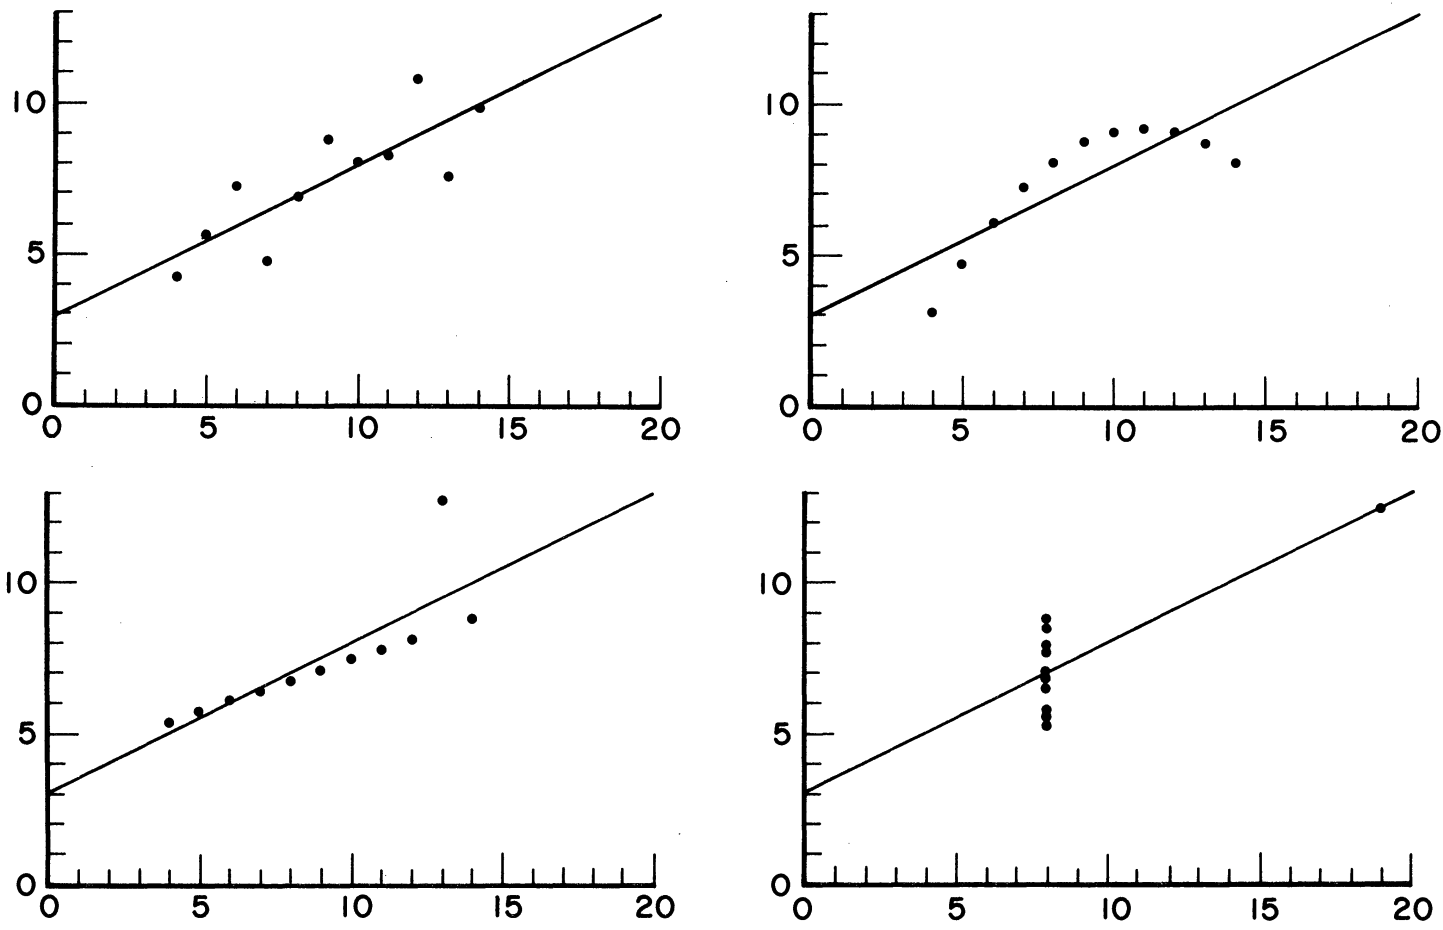
\includegraphics[width=.8\columnwidth]{anscombe}
	\caption[An example showing benefit of visualization]{Four datasets with identical statistics can have very different structures that are easily seen by using simple graphics. \is{Anscombe1973}}
	\label{fig:lr-anscombe}
\end{figure}

For a much larger and more complex dataset, a naive visual representation of the entire dataset often leads to a messy and ineffective visualization. In this case, analysis techniques in machine learning and data mining can be complemented such as applying a clustering method to aggregate data into a representative and more manageable set before visualizing it. The combination of interactive visualization and automated data analysis sets the foundation for the field \emph{visual analytics}~\cite{Keim2008}. In the pioneering book \emph{Illuminating the Path} by Thomas and Cook~\cite{Thomas2005}, with a human sensemaking emphasis, visual analytics is defined as ``the science of analytical reasoning facilitated by interactive visual interfaces''. Keim~et~al.~\cite{Keim2010} suggest a process model for visual analytics as in \autoref{fig:lr-visual-analytics-process} with interactive visualization and data analysis model as the two main components to transform data input to knowledge output.

\begin{figure}
	\centering
	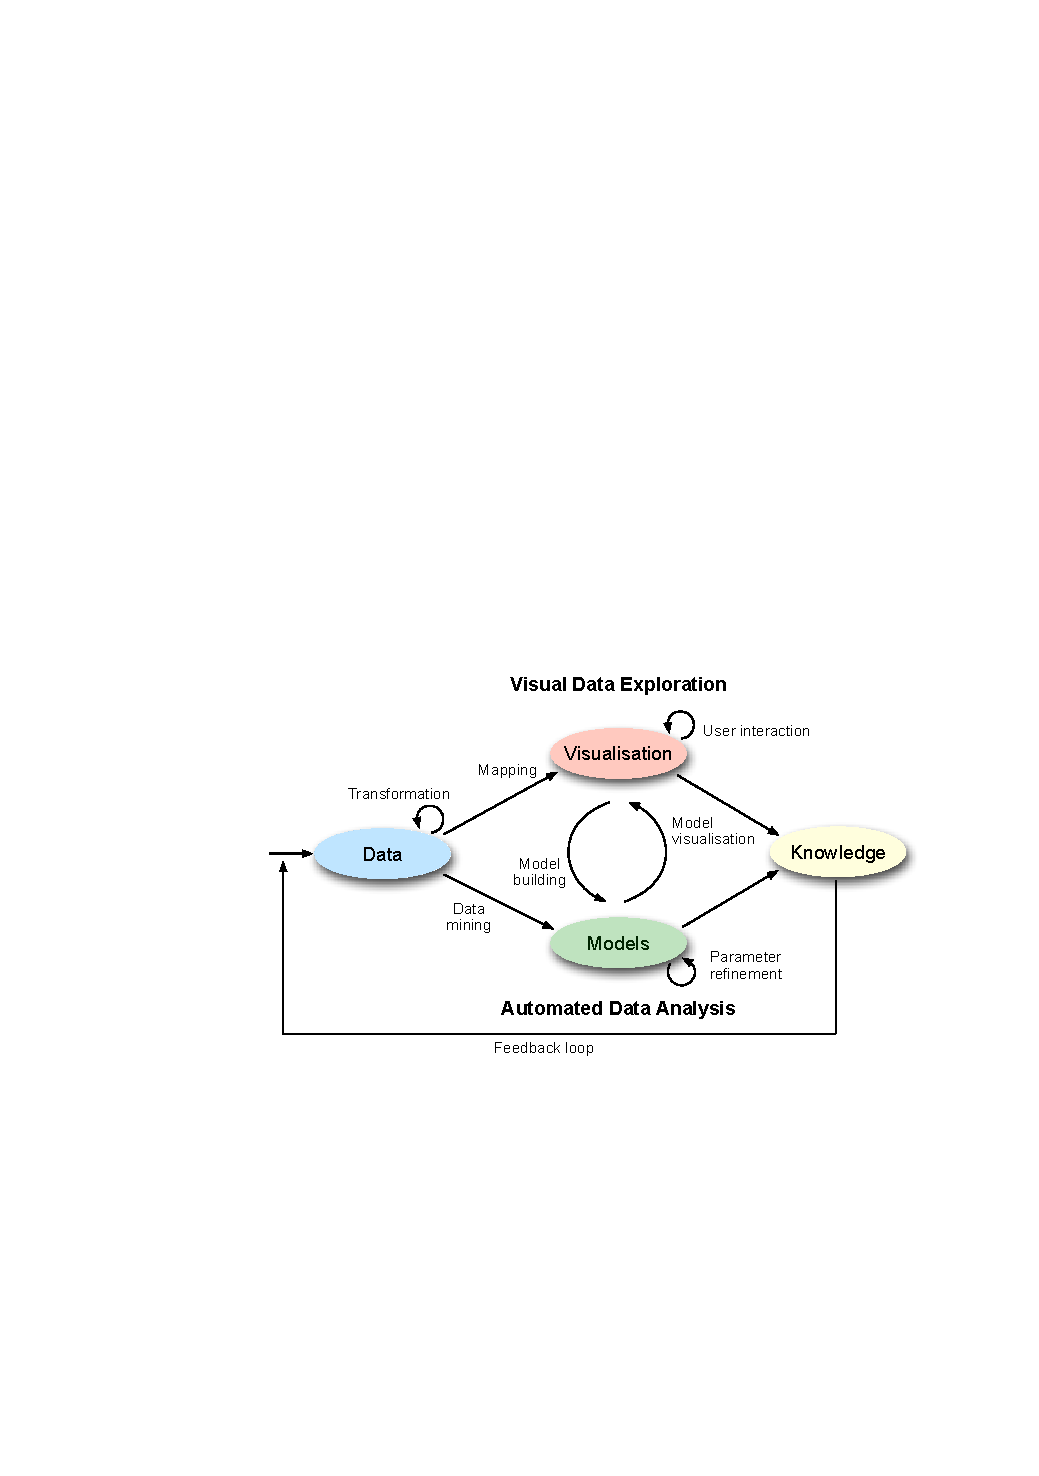
\includegraphics[width=.9\columnwidth]{visual-analytics-process}
	\caption[An iterative visual analytics process model]{An iterative visual analytics process model. It centers around the interaction between data, visualization, models about the data and the users in order to produce knowledge. \is{Keim2010}}
	\label{fig:lr-visual-analytics-process}
\end{figure}

Next, we will review the core work in interactive visualization (\autoref{sub:lr-visualization}) and automated data analysis (\autoref{sub:lr-analysis}). An essential part in every visualization and visual analytics system is to perform validation to check whether the product meets its design purposes and to understand how it helps or hinder users, which will be discussed in \autoref{sub:lr-evaluation}.

\subsection{Visualization Design}
\label{sub:lr-visualization}

This section discusses common principles in designing visual representations of data and common interaction techniques.

\subsubsection{Visual Design Principles}
\label{sub:lr-design}

\paragraph{Marks and Channels}
Marks are basic geometric elements that depict items or links, and channels control their appearance~\cite{Munzner2014}. The number of dimensions in item marks can be zero as a \emph{point}, one as a \emph{line}, two as an \emph{area}, and three as a \emph{volume}. Link marks include \emph{connection} showing a pairwise relationship between two items using a line and \emph{containment} showing hierarchical relationship using areas.

%\autoref{fig:lr-marks} illustrates these marks.

%\begin{figure}
%	\centering
%	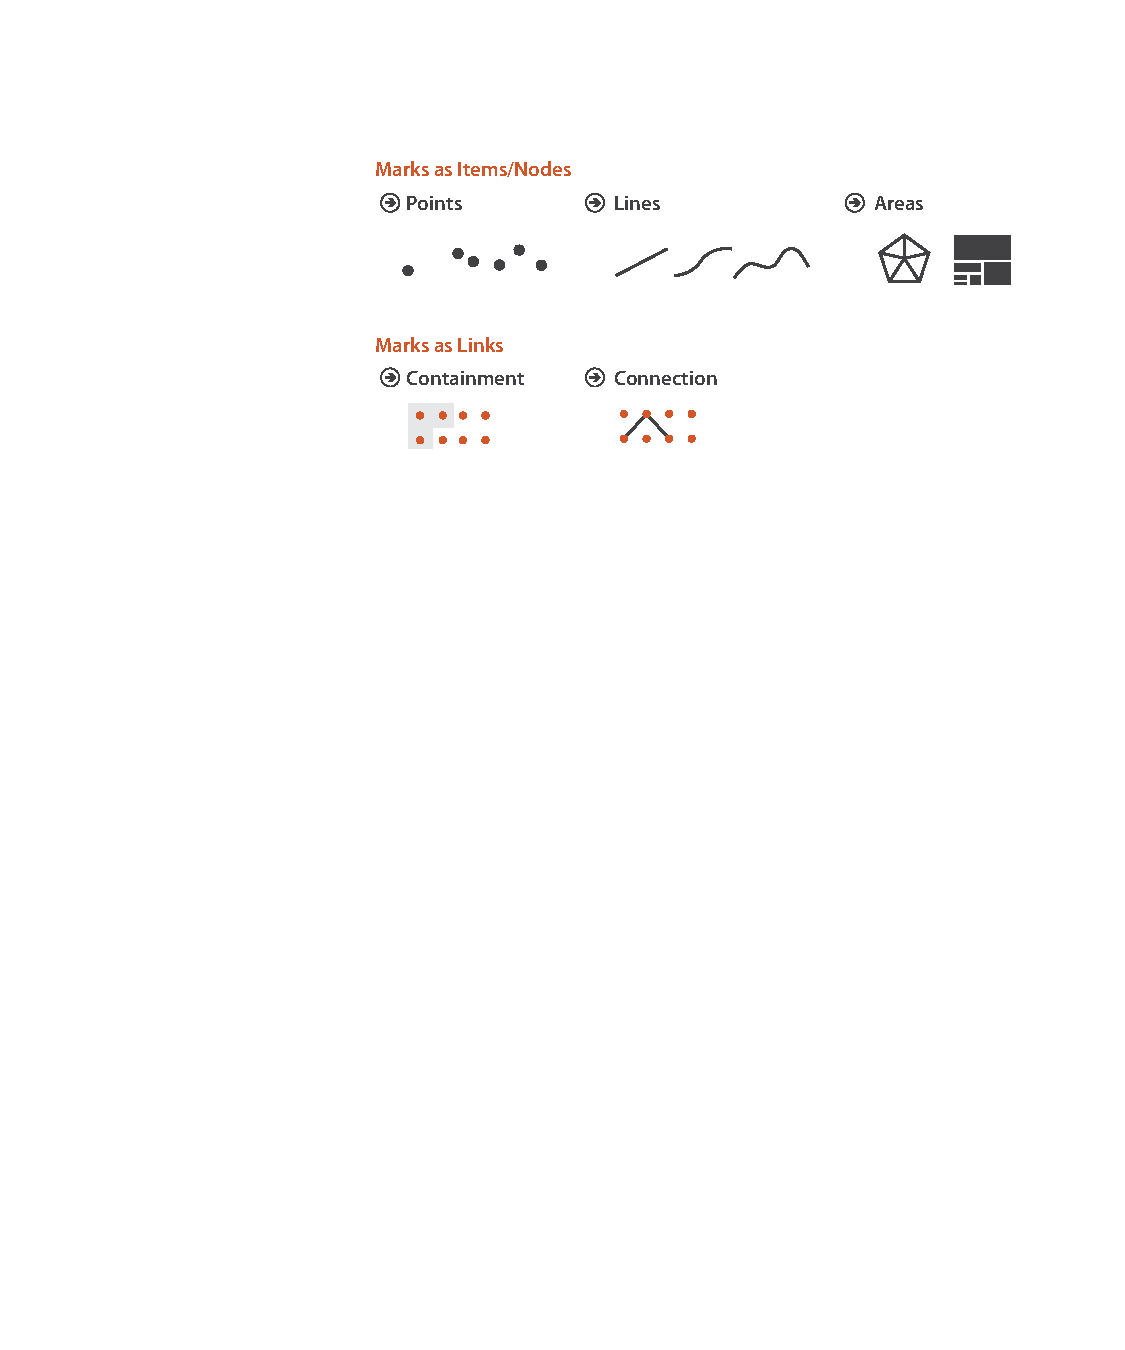
\includegraphics[width=.8\linewidth]{marks}
%	\caption{Item and link marks as geometric primitives. \is{Munzner2014}}
%	\label{fig:lr-marks}
%\end{figure}

A visual channel or graphical attribute controls the appearance of marks such as position, color, shape, angle and size. However, not all channels can be applied to all marks. For instance, an area mark can be used in a geographic map to denote a region. Because the area mark (as a geographic region) is already associated with a shape, it cannot be size-coded to represent another quantitative attribute.
All channels are not equal; they are processed and perceived differently by our human visual systems. Also, not all channels are appropriate for encoding both ordered and non-ordered attributes. Ordered attributes should be shown using magnitude channels, with \emph{aligned spatial position} as the most effective channel and \emph{3D volume} as the least effective one. Categorical (non-ordered) attributes should be shown using identity channels, with \emph{spatial region} as the most effective channel and \emph{shape} as the least effective one. Munzer's book~\cite{Munzner2014} describes the detailed ranking of effectiveness of visual channels, which is based on empirical studies such as the work by Cleveland and McGill~\cite{Cleveland1985}, and by Heer and Bostock~\cite{Heer2010a}.

Color is an interesting channel that can be used for both data attribute types. Color luminance and saturation are used for magnitude channels, and color hue is used for identity channels. A colormap specifies a mapping between colors and data values, and designing such an effective colormap is challenging. ColorBrewer~\cite{Harrower2003} is an excellent source for colormap reference, providing color schemes for both ordered and categorical attributes. Human can only distinguish around 12 colors at the same time~\cite{Munzner2014}. \autoref{fig:lr-colorbrewer-1} shows such a categorical colormap with 12 distinguished color hues. Ordered colormaps can be either sequential (\autoref{fig:lr-colorbrewer-2}) or diverging (\autoref{fig:lr-colorbrewer-3}). Diverging colormaps use two different color hues to emphasize values below and above the middle point.

\begin{figure}
	\centering
	\subcaptionbox{Categorical colormap with distinguishable color hues.\label{fig:lr-colorbrewer-1}}[\columnwidth]{
\includegraphics[height=.07\columnwidth]{colorbrewer-1}}
	\\
	\subcaptionbox{Sequential colormap: a single color hue with different saturation level.\label{fig:lr-colorbrewer-2}}[\columnwidth]{\hspace{-.11\columnwidth}
\includegraphics[height=.07\columnwidth]{colorbrewer-2}}
	\\
	\subcaptionbox{Diverging colormap: two color hues emphasizing positive and negative values.\label{fig:lr-colorbrewer-3}}[\columnwidth]{\hspace{-.045\columnwidth} 
\includegraphics[height=.07\columnwidth]{colorbrewer-3}}
	\caption[Colormaps from ColorBrewer]{Colormaps from ColorBrewer. \is{Harrower2003}}
\end{figure}

\paragraph{Gestalt Principles}
\label{sub:lr-gestalt}
Gestalt principles describe how people see patterns in visual display~\cite{Koffka1935}. This section reviews three commonly used Gestalt principles.

\subparagraph{Similarity}
Similar elements tend to be perceived as a group. \autoref{fig:lr-gestalt-similarity-1} shows a matrix of point marks with uniform spacing, but using two different shapes: dot and cross. The similarity of shapes helps us see the rows more clearly than the columns. Two separable channels can be applied together to reveal patterns by either rows or columns. In \autoref{fig:lr-gestalt-similarity-2}, color (green) is used to depict rows, and texture is used to depict columns.

\begin{figure}
	\centering
	\subcaptionbox{Similarity of shapes distinguishes rows.\label{fig:lr-gestalt-similarity-1}}[.47\columnwidth]{
\includegraphics[height=.25\columnwidth]{gestalt-similarity-1}}
	\hfill
	\subcaptionbox{Color and texture delineate rows and columns, respectively.\label{fig:lr-gestalt-similarity-2}}[.47\columnwidth]{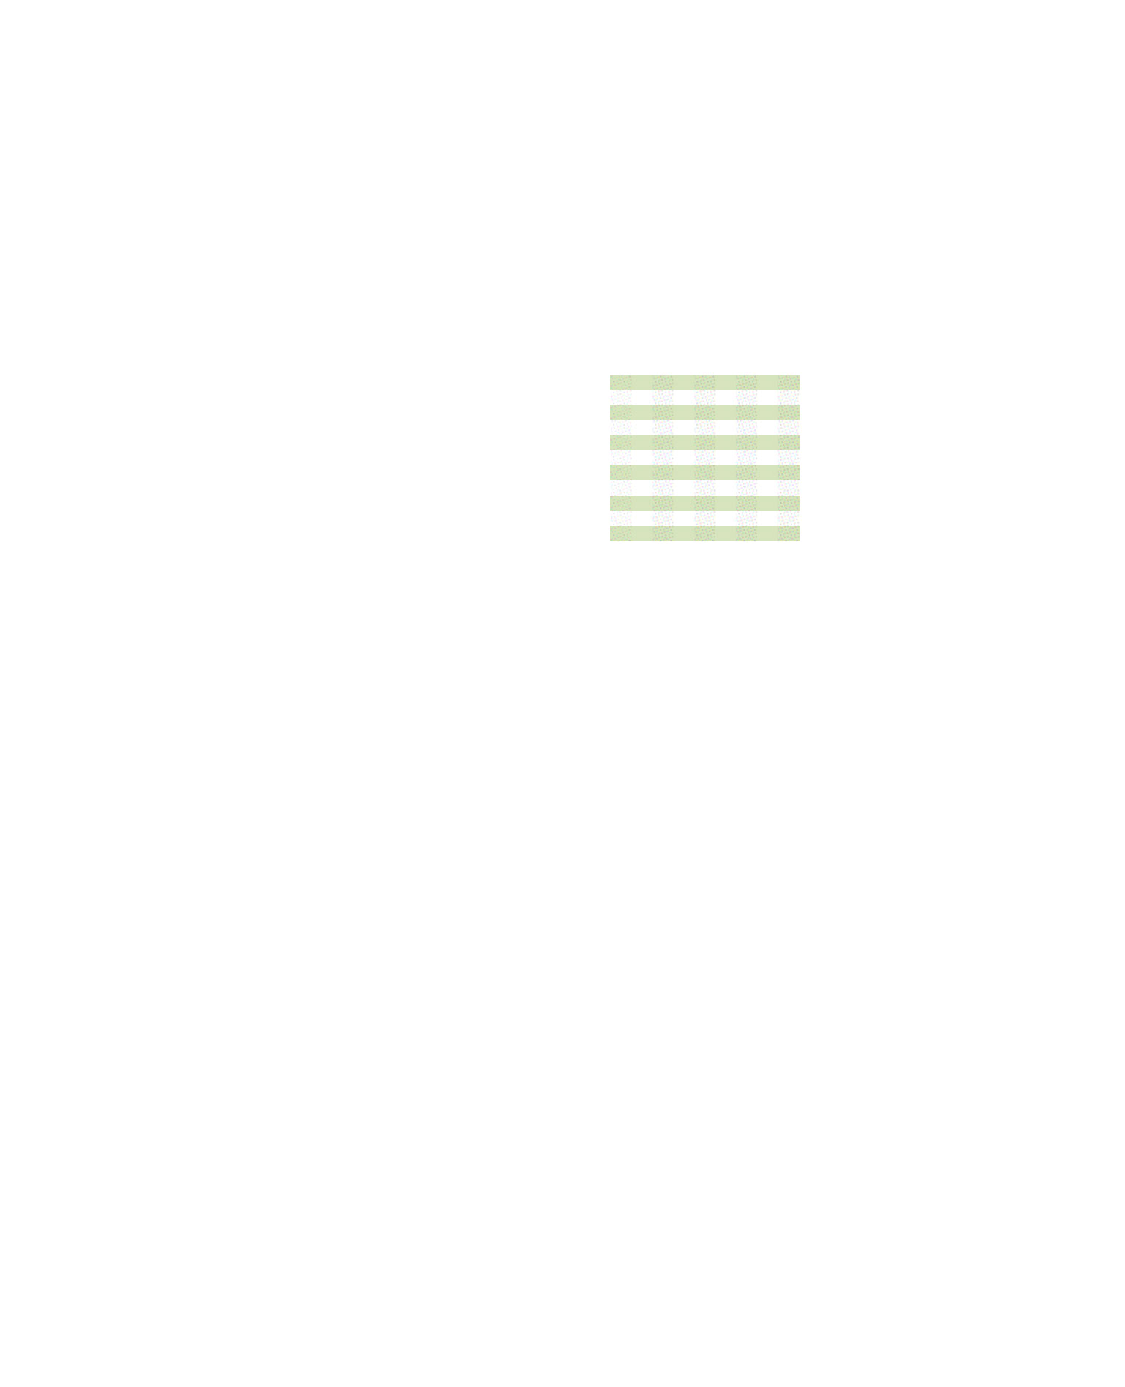
\includegraphics[height=.25\columnwidth]{gestalt-similarity-2}} \label{fig:lr-gestalt-similarity}
	\caption[Similarity principle]{Similarity principle: similar elements are perceived as a group. \is{Ware2013}}
\end{figure}

\subparagraph{Proximity}
Elements that are close together are perceptually grouped together. \autoref{fig:lr-gestalt-proximity-1} shows two clear groups of dots. \autoref{fig:lr-gestalt-proximity-2} shows rows of dots. However, with a small change of spacing, these dots are perceived as columns in \autoref{fig:lr-gestalt-proximity-3}. The application of this principle is straightforward: organizing related information close together. It helps separate groups of unrelated objects and facilitates searching for information.

\begin{figure}
	\centering
	\subcaptionbox{Two groups of dots.\label{fig:lr-gestalt-proximity-1}}[.3\columnwidth]{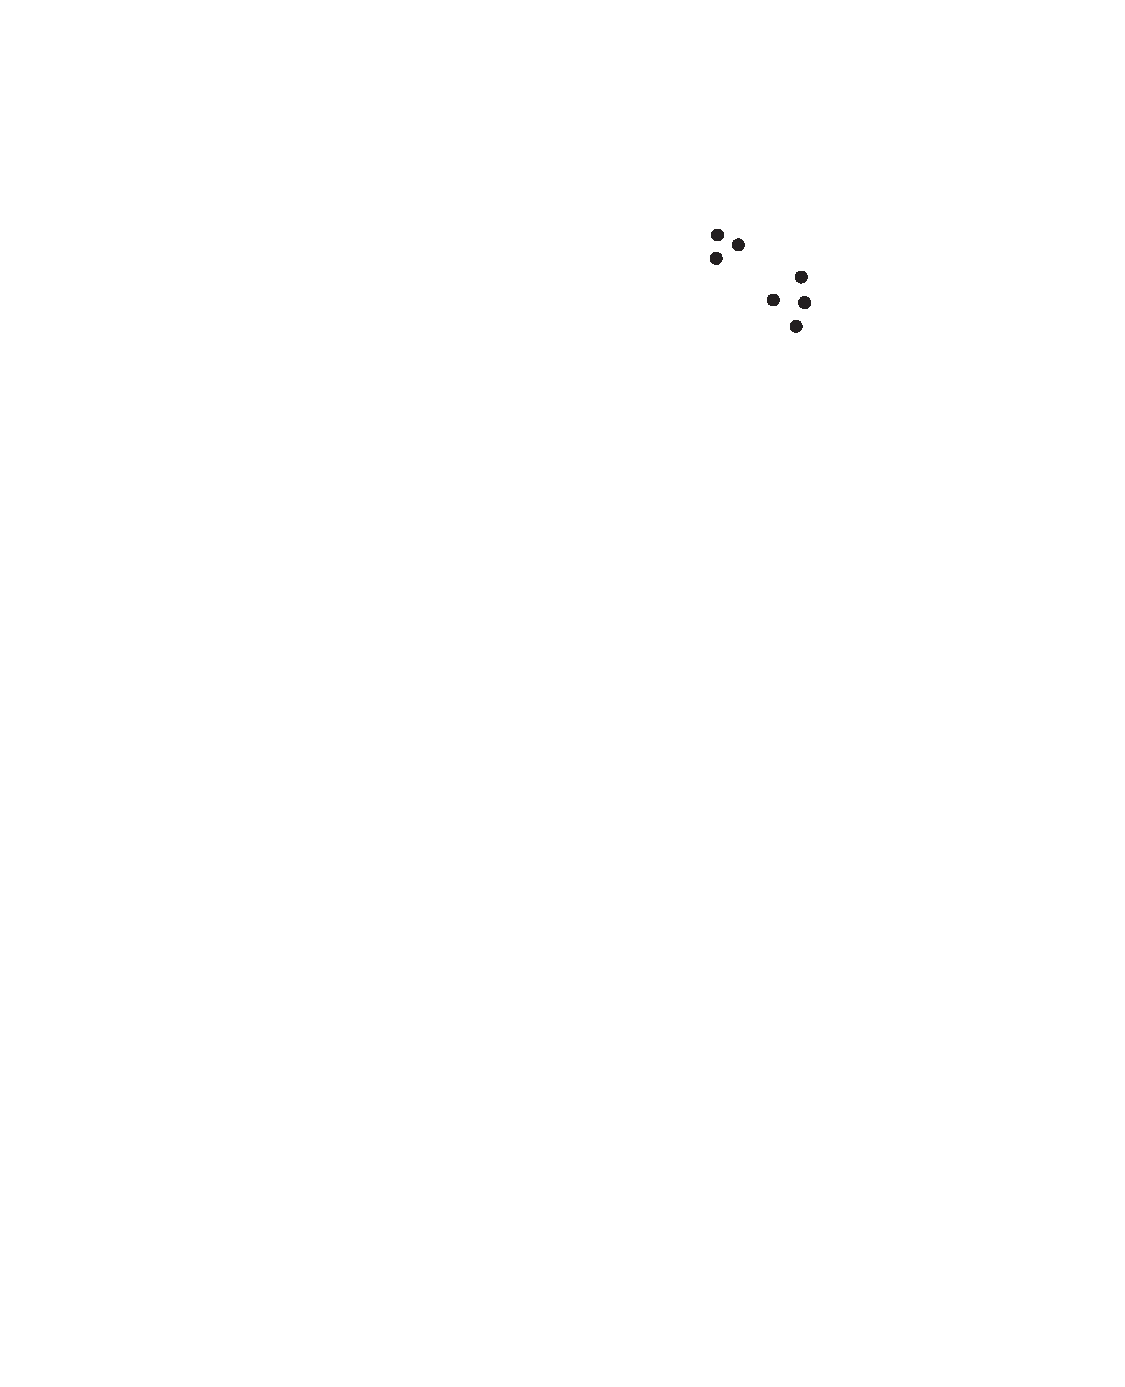
\includegraphics[width=.15\columnwidth]{gestalt-proximity-1}}
	\hfill
	\subcaptionbox{Rows of dots.\label{fig:lr-gestalt-proximity-2}}[.3\columnwidth]{
\includegraphics[width=.25\columnwidth]{gestalt-proximity-2}}
	\hfill
	\subcaptionbox{Columns of dots.\label{fig:lr-gestalt-proximity-3}}[.3\columnwidth]{
\includegraphics[width=.25\columnwidth]{gestalt-proximity-3}}
	\label{fig:lr-gestalt-proximity}
	\caption[Spatial proximity principle]{Spatial proximity principle: spatially close elements are perceived as a group. \is{Ware2013}}
\end{figure}

\subparagraph{Connectedness}
Elements that are connected by visual properties are perceived as being more related than elements that are not connected. This principle can be achieved simply by drawing a border around a group of elements as in \autoref{fig:lr-gestalt-connectedness-1}. This is extensively applied in designing complex graphical user interface: groups of related features are separated by borders. Another way to achieve connectedness is by drawing lines between related elements as in \autoref{fig:lr-gestalt-connectedness-2}. This is the basics of \emph{node-link diagrams} -- one of the most common methods of representing relationships between elements.

\begin{figure}
	\centering
	\subcaptionbox{Using border to denote a group.\label{fig:lr-gestalt-connectedness-1}}[.47\columnwidth]{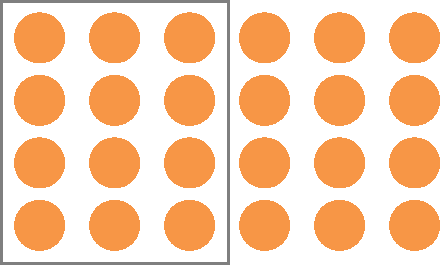
\includegraphics[width=.25\columnwidth]{gestalt-connectedness-1}}
	\hfill
	\subcaptionbox{Using lines to denote a group.\label{fig:lr-gestalt-connectedness-2}}[.47\columnwidth]{
\includegraphics[width=.25\columnwidth]{gestalt-connectedness-2}}
	\caption[Connectedness principle]{Connectedness principle: visually connected elements are perceived as a group. \is{Ware2013}}
	\label{fig:lr-gestalt-connectedness}
\end{figure}

Among these three principles, connectedness has the strongest effect, followed by proximity and then similarity. \autoref{fig:lr-gestalt} illustrates this comparison. In \autoref{fig:lr-gestalt-1}, even though spacing between dots in rows is shorter than spacing between dots in columns, the connected lines make the vertical links has a stronger grouping effect than rows. In \autoref{fig:lr-gestalt-2}, the lines also make the horizontal links more notable than groups of colored circles. In \autoref{fig:lr-gestalt-3}, two spatial groups are more clearly perceived than colored groups.

\begin{figure}
	\centering
	\subcaptionbox{Links are perceived more clearly than spatial groups.\label{fig:lr-gestalt-1}}[.3\columnwidth]{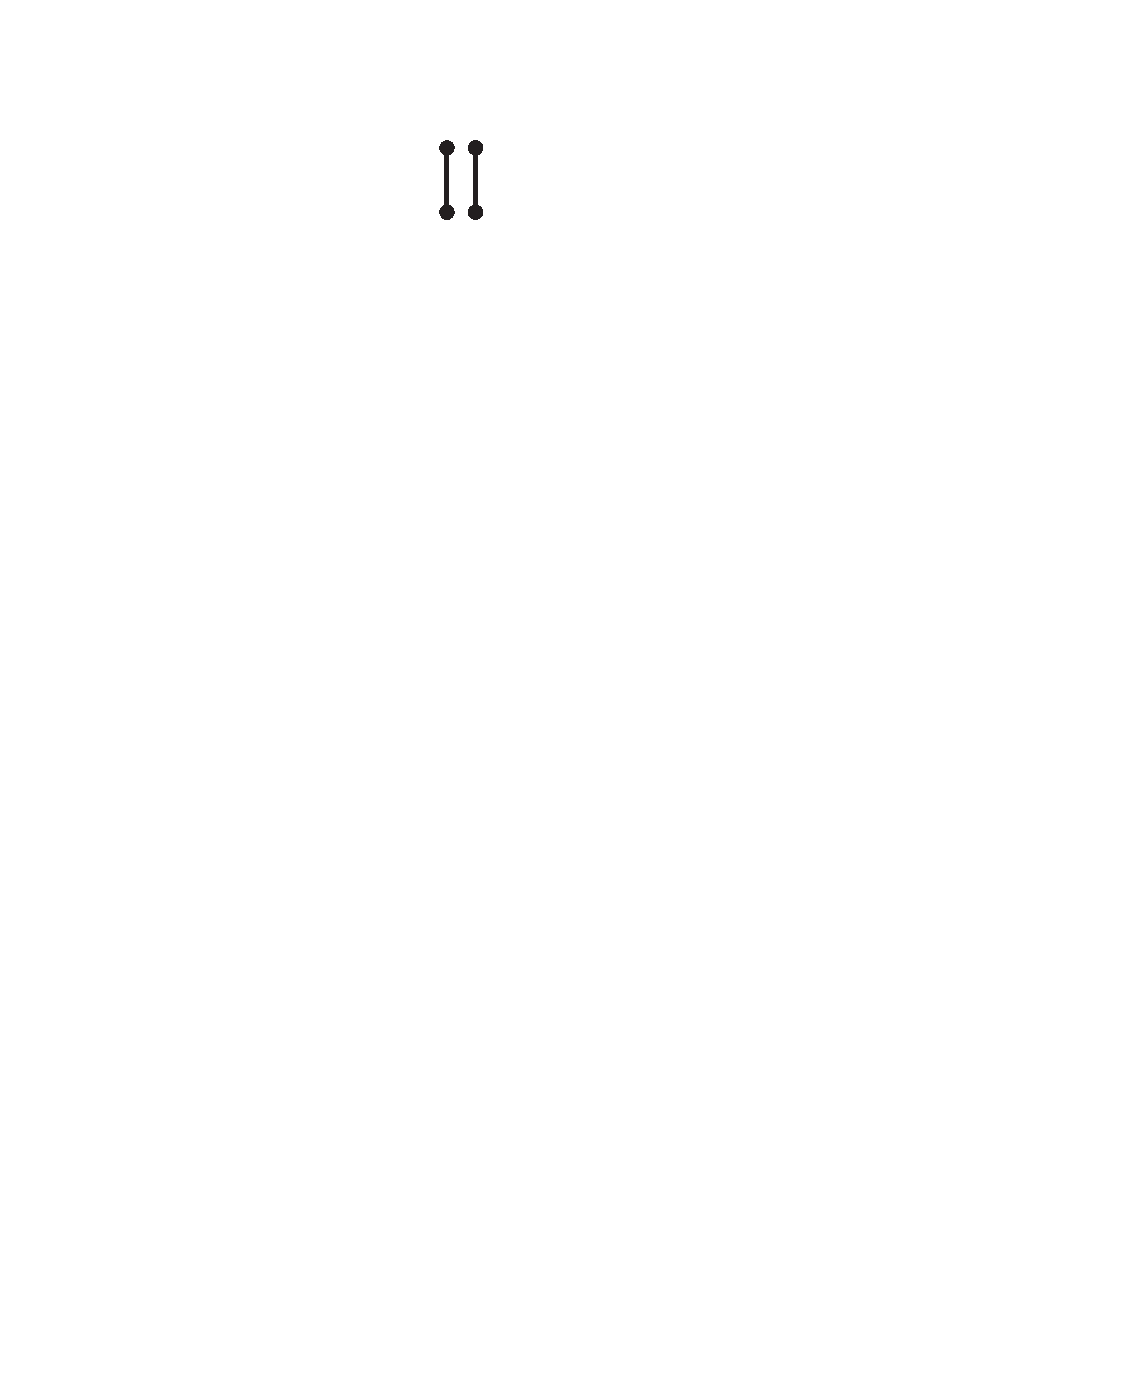
\includegraphics[height=.08\columnwidth]{gestalt-1}}
	\hfill
	\subcaptionbox{Links are perceived more clearly than colored groups.\label{fig:lr-gestalt-2}}[.3\columnwidth]{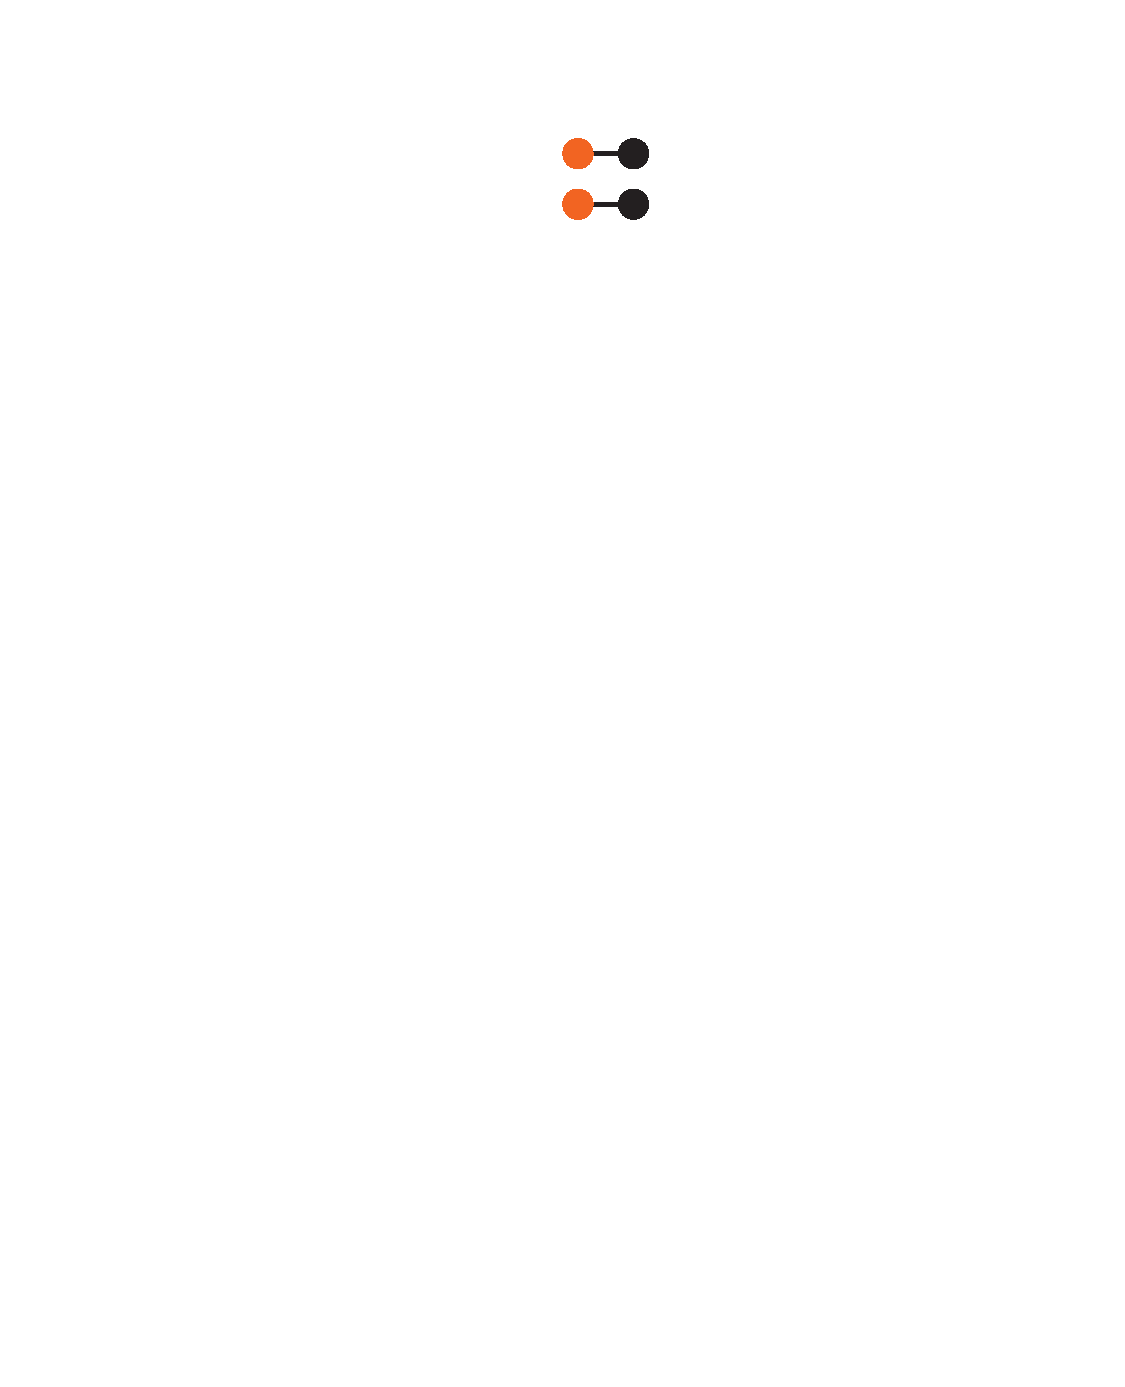
\includegraphics[height=.08\columnwidth]{gestalt-2}}
	\hfill
	\subcaptionbox{Spatial groups are perceived more clearly than colored groups.\label{fig:lr-gestalt-3}}[.3\columnwidth]{
\includegraphics[height=.08\columnwidth]{gestalt-3}}
	\caption[Comparison of Gestalt principles]{Comparison of Gestalt principles. Connectedness is stronger than proximity, and proximity is stronger than similarity. \is{Ware2013}}
	\label{fig:lr-gestalt}
\end{figure}

\paragraph{Tufte's Principles}
Tufte proposes a number of principles in designing effective graphics in his series of books, most notably including \emph{The Visual Display of Quantitative Information}~\cite{Tufte1983} and \emph{Envisioning Information}~\cite{Tufte1990}. This section reviews three principles that have been commonly applied in graphic design and visualization.

\subparagraph{Graphical Integrity}
This principle emphasizes that the graphical representation should tell the truth about the data. Representation of numbers, as physically measured on the surface of the graphic itself,	must be directly proportional to the numerical quantities represented. \autoref{fig:lr-tufte-integrity-1} shows a falsely big drop in stock market value between 2001 and 2002. It is because the chart uses a relative scale with the value range from 450 to 500, causing its height disproportional to the market value. \autoref{fig:lr-tufte-integrity-2} corrects this error by using an absolute scale with the value range starting from 0.

\begin{figure}
	\centering
	\subcaptionbox{Using a relative value range causes a falsely big drop of stock market value between 2001 and 2002.\label{fig:lr-tufte-integrity-1}}[.47\columnwidth]{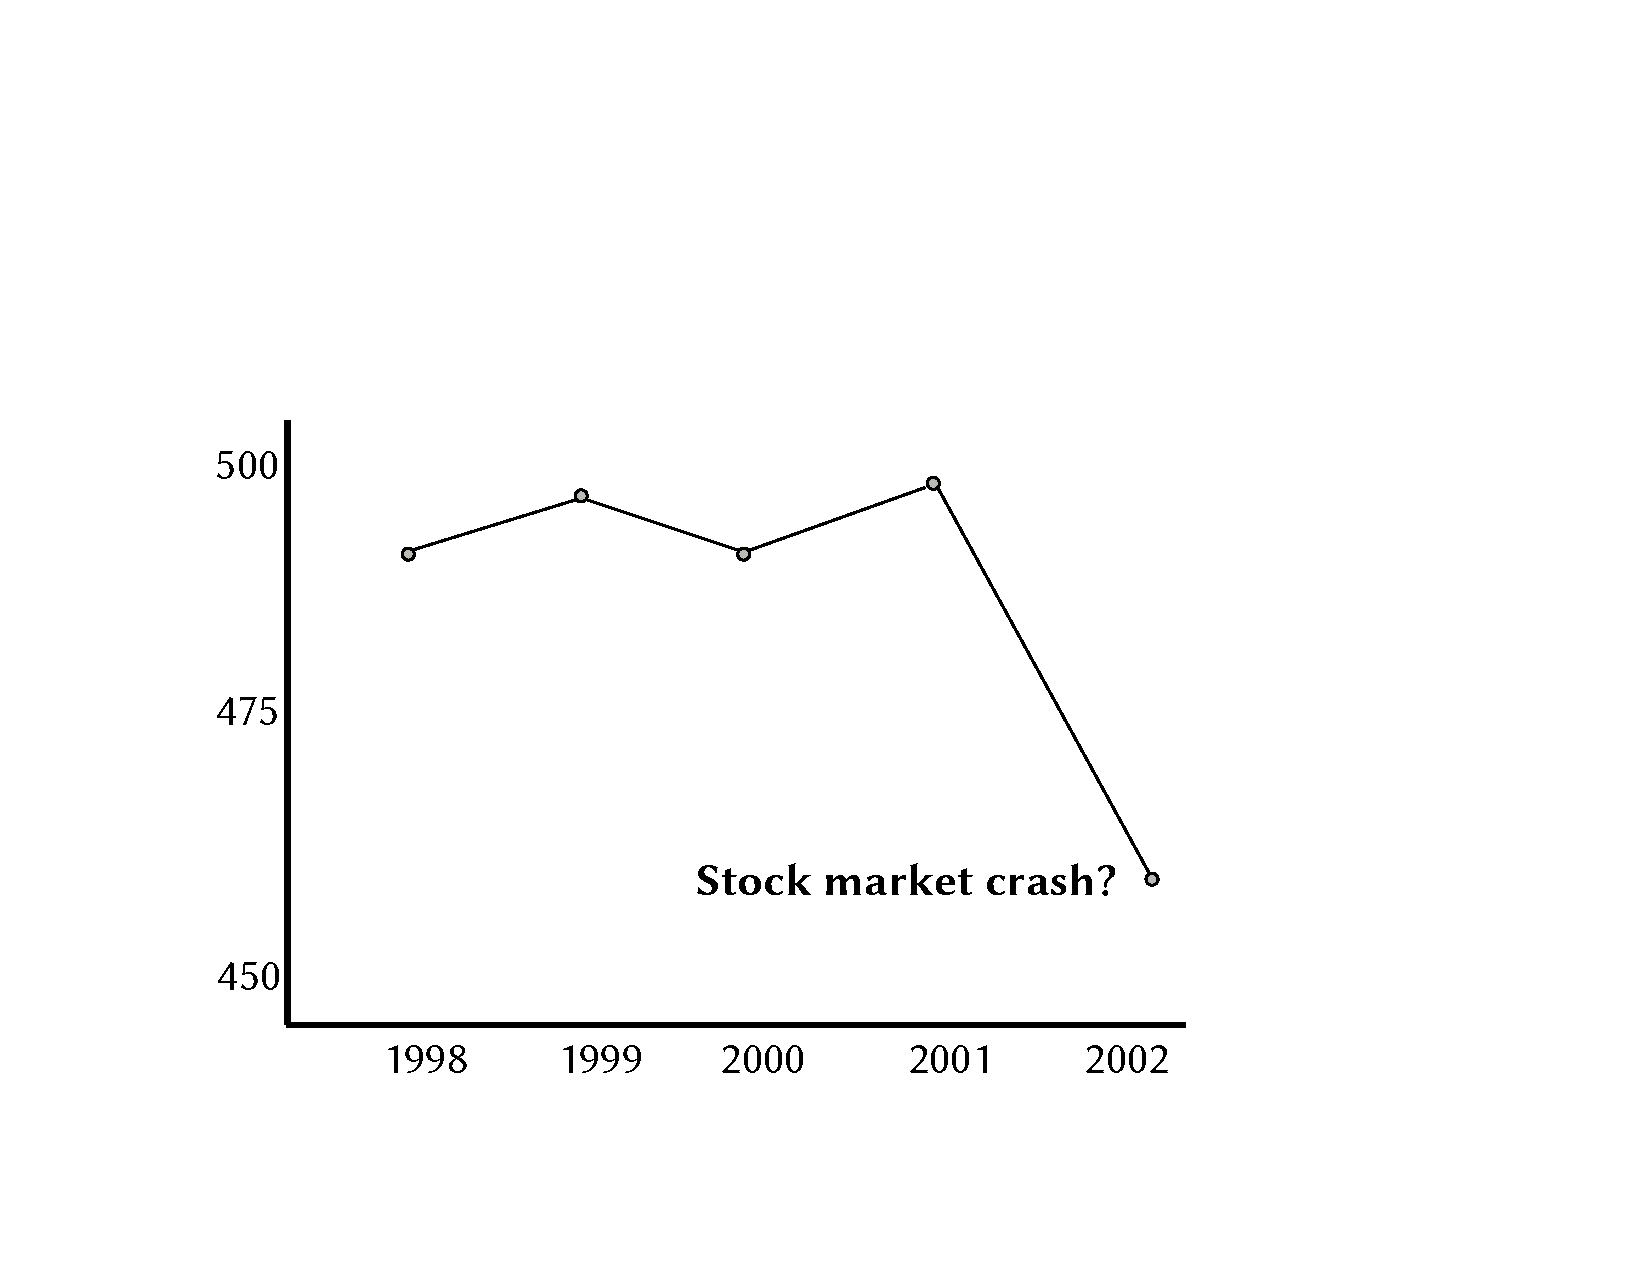
\includegraphics[width=.47\columnwidth]{tufte-integrity-1}}
	\hfill
	\subcaptionbox{Using an absolute value range to depict the data accurately.\label{fig:lr-tufte-integrity-2}}[.47\columnwidth]{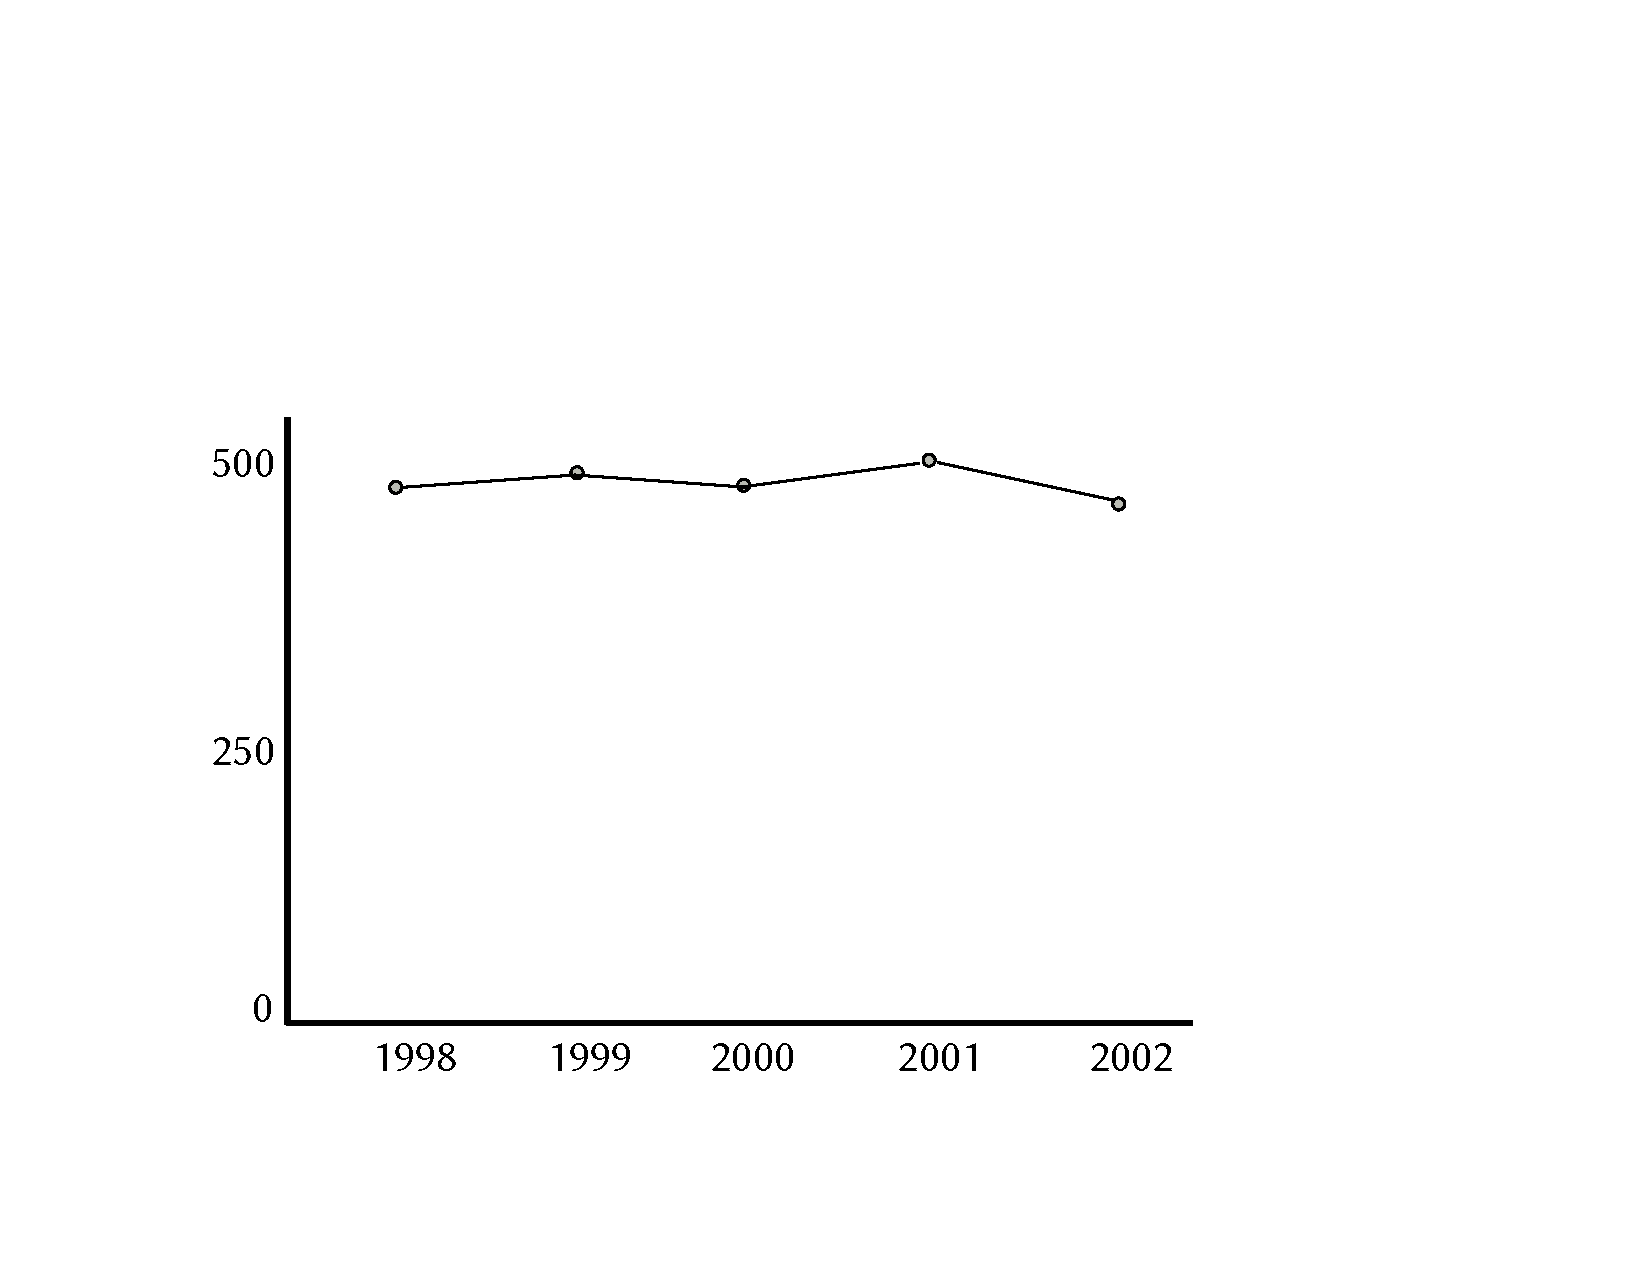
\includegraphics[width=.47\columnwidth]{tufte-integrity-2}}
	\caption[Graphical integrity principle]{Graphical integrity principle. The chart should tell the truth about the data.}
	\label{fig:lr-tufte-integrity}
\end{figure}

\begin{figure}
	\centering
	\subcaptionbox{A bar chart with poor data-ink ratio.\label{fig:lr-tufte-ink-1}}[.47\columnwidth]{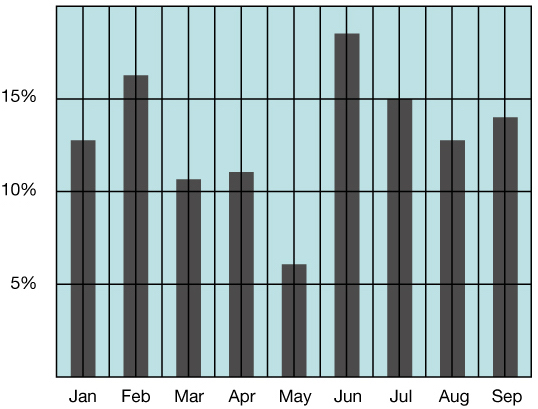
\includegraphics[width=.47\columnwidth]{tufte-ink-1}}
	\hfill
	\subcaptionbox{A bar chart with high data-ink ratio by removing background, border and grid lines.\label{fig:lr-tufte-ink-2}}[.47\columnwidth]{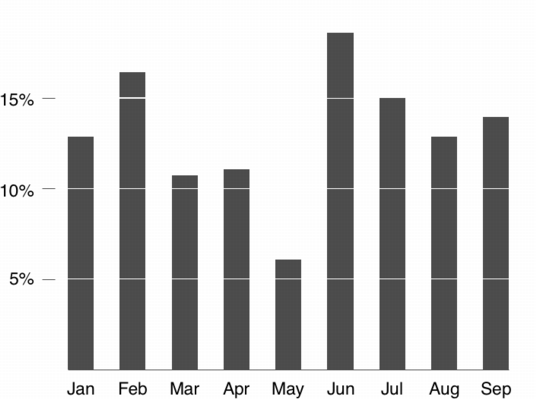
\includegraphics[width=.47\columnwidth]{tufte-ink-2}}
	\caption[Data-ink ratio maximization principle]{Data-ink ratio maximization principle: removing the graphic that does not contribute to the understanding of the data.}
	\label{fig:lr-tufte-ink}
\end{figure}
% Source: http://www.infovis-wiki.net/index.php/Data-Ink_Ratio

\subparagraph{Data-Ink Ratio Maximization}
Data-ink includes the pixels in the graphic that are used for representing the data. Data-ink ratio is defined as the ratio between the data-ink and the total non-background pixels used in the graphic. This principle aims to maximize this ratio by erasing non-data-ink and erasing redundant data-ink. \autoref{fig:lr-tufte-ink} illustrates this principle.

\subparagraph{Micro/Macro Readings}
This principle suggests that a graphic can contain both enormous details and an overall pattern. This allows the viewer to glance from a distance to observe the big picture before drilling-down closely to examine its individual pieces. Classic stem-and-leaf plot is a great example of this principle (\autoref{fig:lr-tufte-micro}). The plot shows all individual data items at an understandable level of detail, and from an overview, it provides the data distribution. The micro/macro principle is extensively applied in interactive visualization, where zooming and panning are made possible.

\begin{figure}
	\centering
	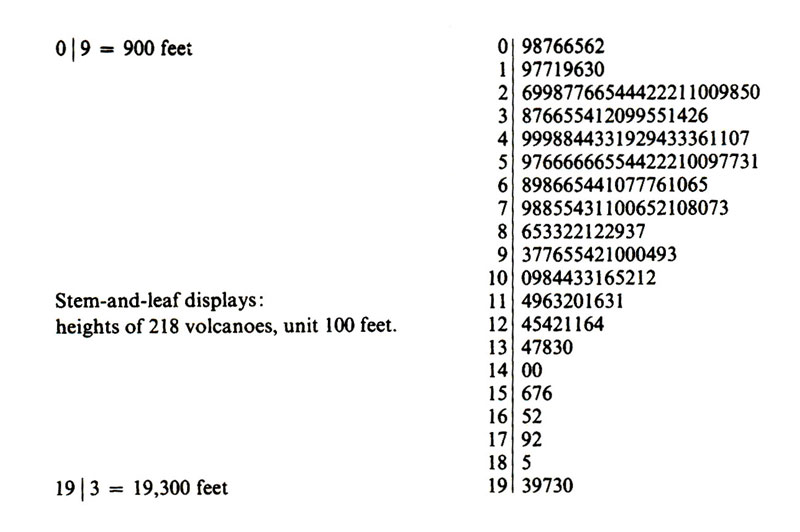
\includegraphics[width=.6\linewidth]{tufte-micro}
	\caption[Micro/macro principle]{Micro/macro principle. A stem-and-leaf plot shows both the data distribution and individual items. Data shows heights of 218 volcanoes, unit 100 feet. \is{Tufte1983}}
	\label{fig:lr-tufte-micro}
\end{figure}


%In a broader context, GUI design principles:  Schneiderman~\cite{Shneiderman2016} (eight golden rules), Norman (six design principles) ~\cite{Norman2002} and	Nielsen (ten usability heuristics)~\cite{Nielsen1994} -- create a table with rows showing similar principles
%http://www.csun.edu/science/courses/671/bibliography/preece.html
%https://faculty.washington.edu/jtenenbg/courses/360/f04/sessions/schneidermanGoldenRules.html
%https://www.interaction-design.org/literature/article/shneiderman-s-eight-golden-rules-will-help-you-design-better-interfaces

\subsubsection{Interaction Techniques}
Interaction typically refers to the set of controls provided to the user to manipulate an interface~\cite{Pike2009a}. A static visualization can only show one aspect from a dataset. When the dataset is large enough, showing all the data at once may also make the visualization become cluttered. Interaction plays an important role in addressing this problem. It can help explore large datasets at multiple levels of detail, identify patterns through examination of different visual representations, and understand the connections between them.

Examples of interaction include standard techniques commonly used in graphical user interface such as mouse clicking and scrolling, and more visualization specific techniques such as \emph{linking and brushing}~\cite{Kosara2003}. Commonly, a visualization consists of multiple views, each showing an aspect of the dataset. These views should be linked together to best exploit their strengths. The user can select points of interest using the brushing technique, typically done directly on the visual data representation such as dragging a rectangular area. Besides spatial selection, data can also be selected by data-related similarity with a given point such as all items having the same given attribute value~\cite{Heer2008a}. The data points are brushed in one view and are highlighted in other views, allowing the user to explore them with different perspectives and representations (\autoref{fig:lr-linking}).

\begin{figure}
	\centering
	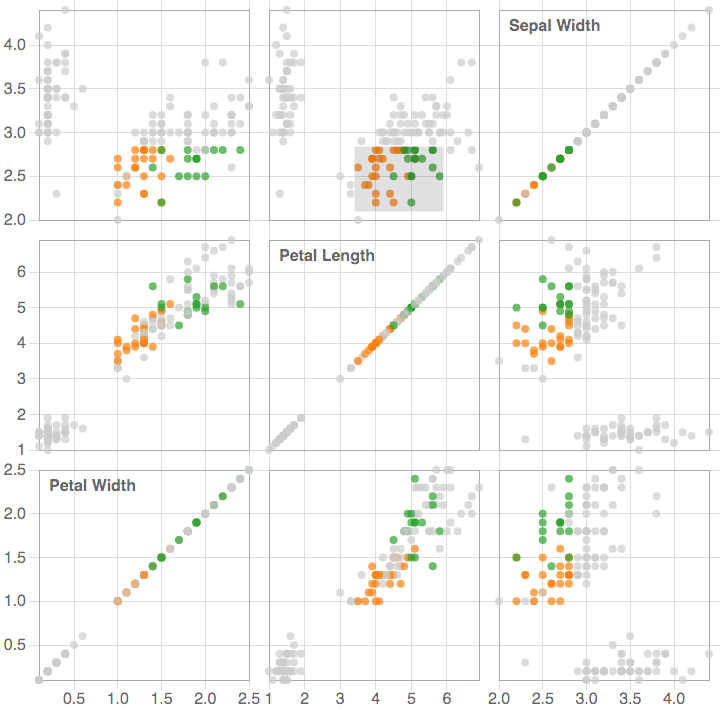
\includegraphics[width=.7\columnwidth]{linking}
	\caption[Linking and brushing]{Linking and brushing. Data points brushed in one view are linked and highlighted in other views.}
	\label{fig:lr-linking}
\end{figure}

Many approaches are proposed to visualize a large amount of information such as overview and detail~\cite{Cockburn2008} and semantic zooming~\cite{Perlin1993}. The former method uses two views: one to see the current detail and one to keep track of its global context. This is analogous to the world we can see and its geographic map. The later method uses a single view but with representations for different levels of detail. It lets the user to adjust zoom level to explore the information of interest. Focus+Context is another technique that brings both the overview (context) and the detailed information (focus) together in one view. Fisheye~\cite{Furnas1986,Furnas2006} is one example of this technique: the focal region is magnified and displayed within its surrounding context (\autoref{fig:lr-fisheye}). For all these techniques, interaction is the key factor allowing the user to navigate through a large amount of information and examine the one of interest.

\begin{figure}
	\centering
	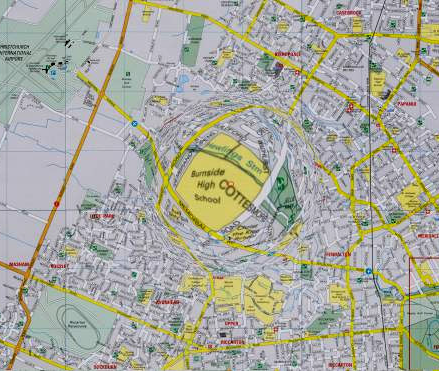
\includegraphics[width=.7\columnwidth]{fisheye}
	\caption[Fisheye view for focus+context]{Fisheye view for focus+context. Both the overview and the detailed information are displayed in one view. \is{Cockburn2008}}
\label{fig:lr-fisheye}
\end{figure}

Taxonomies of interaction techniques by type include the work by Dix and Ellis~\cite{Dix1998}, by Keim~\cite{Keim2002}, and by Wilkinson~\cite{Wilkinson2005}. Very often, a user performs a particular interaction (or a series of them) to achieve some goal, thus interaction techniques can also be classified based on their intent. Different interaction techniques in different visualizations may actually serve the same purpose. For example, both drilling-down in a treemap~\cite{Shneiderman1992} and semantic zooming aim to get more details. Taxonomies of high-level interaction can be found in the work by Yi~et~al.~\cite{Yi2007}, by Heer and Shneiderman~\cite{Heer2012}, and by Brehmer and Munzner~\cite{Brehmer2013}. These classifications could help visualization designers select suitable interaction techniques to serve for the capabilities they want to offer to the users.

%Several methods can improve existing different interaction techniques.
Traditional graphical user interface widgets are often used to control different settings of a visualization, such as buttons and sliders. Its disadvantage is that visual feedback does not appear where the interaction happens, but elsewhere in the visualization. It also takes time for the user to search for the appropriate setting controllers. Direct manipulation~\cite{Shneiderman1982} of visualization is an approach to address this problem. It enables the user to directly interact with the visual representation and receive immediate feedback. One example is that the axes of a parallel coordinates plot can be reordered by direct dragging and values can be filtered by direct brushing on the axes (\autoref{fig:lr-pcp}). Surrogate objects can be effective when the data objects are small or distant, thus difficult to manipulate~\cite{Kwon2011}. An example is the use of interactive legends as filtering means~\cite{Riche2010b}.

\begin{figure}
	\centering
	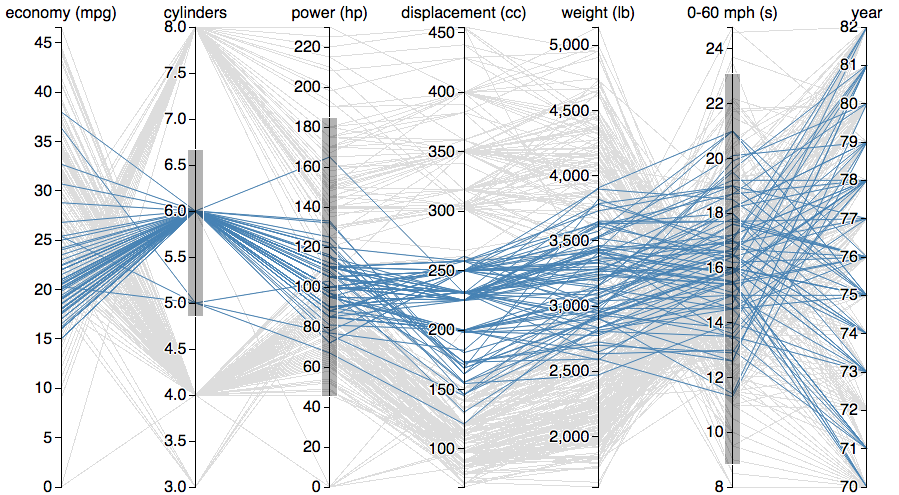
\includegraphics[width=.8\linewidth]{pcp}
	\caption[Direct manipulation in a parallel coordinates plot]{Direct manipulation in a parallel coordinates plot with reorder-able and brush-able axes.}
	\label{fig:lr-pcp}
\end{figure}

\emph{Fluid interaction}~\cite{Elmqvist2011} can be applied to improve existing interaction techniques. Besides using direct manipulation as discussed previously, the interaction should produce a smooth animated transition between the state before and the state after an interaction, helping users maintain their mental maps. It also needs to provide immediate visual feedback, allowing users to know what is happening and/or what will happen next.

Interaction techniques are often combined to explore the data or explain a known story. A classic visual information-seeking mantra proposed by Shneiderman~\cite{Shneiderman1996} summarizes many information design guidelines and interaction techniques for designing effective information visualizations: \emph{Overview first, zoom and filter, then details-on-demand}. With large datasets, it is challenging to create an overview and provide cues for further exploration. A more suitable approach in this case is \emph{Search, show context, expand on demand}~\cite{VanHam2009}.

\subsection{Automated Analysis Techniques}
\label{sub:lr-analysis}
Data mining is a computational process of extracting patterns in large datasets~\cite{Tan2006}. Its tasks can be broadly divided into two major categories:

\subparagraph{Descriptive tasks} The objective is to derive patterns (correlations, clusters, trajectories and anomalies) that summarize the underlying relationships in data. Example tasks include cluster and association analyses. \emph{Clustering} aims to split data items to groups such that items within a group are more similar to each other than those in other groups. For example, clustering can be used to help marketers discover distinct groups of their customers before applying appropriate marketing strategies to those groups. \emph{Association} analysis discovers the connections among a set of data items. For example, it can be used to identify products that customers often purchase together such as bread and milk.

\subparagraph{Predictive tasks} The objective is to predict the value of an unknown (target) attribute based on the values of other (explanatory) attributes. Example tasks include classification and regression. \emph{Classification} predicts discrete target variables whereas, \emph{regression} focuses on continuous ones. For example, predicting whether a customer buys a marketing product is a classification task because the target variable is binary. However, estimating a future house price is a regression task because price is a continuous variable.

\vspace{2mm}
\noindent Next, we discuss the clustering and classification tasks in more detail and present how they are applied together with visualization to help users gain deeper insight into the data.

\subsubsection{Clustering}

\paragraph{Overview}
Cluster analysis finds similarities between data points based on their attributes and groups similar data points into clusters. Clustering is regarded as \emph{unsupervised learning}~\cite{Han2011} because it can reveal hidden structure in a dataset that does not have \emph{labels} (or groups) defined. The most common clustering algorithm is \emph{k-means}~\cite{Lloyd1982}. Given a set of data points $(x_1, x_2, \dots, x_n)$, k-means clustering aims to partition them into $k$ clusters $(S_1, S_2, \dots, S_k)$, such that the within-cluster sum of squared distances is minimized:
\[
\sum_{i=1}^k\sum_{x\in S_i} \lVert x-\mu_i \rVert^2
\]
where $\mu_i$ is the center of points or centroids in $S_i$.

The algorithms work as follows. Initially, it partitions data points into $k$ non-empty random subsets. Then, the centroids of the current clusters are computed, and each data point is assigned to the cluster with the nearest centroid. The centroid computation and cluster assignment are repeated until no assignment can be done. This k-means clustering algorithm is efficient but often terminates at a local optimal. More detailed analysis of k-means and other clustering algorithms are beyond the scope of this thesis and can be found in data mining textbooks~\cite{Tan2006,Han2011}.

\paragraph{Application Examples}
Human motion tracking data has been applied in various research fields such as medicine, sports and animation~\cite{Bernard2013}. The data consists of temporal sequences of human poses represented by a set of 3D joint positions (e.g., head, hands, elbows and knees). However, analyzing a large collection of such temporal and high-dimensional datasets is challenging. To gain an overall understanding of the data, MotionFlow~\cite{Jang2016} applies a k-means clustering method using a simple Euclidean distance of 3D joints as the similarity measurement. A cluster of human poses is represented as a glyph with a stick figure showing the centroid of the cluster and semi-transparent ghosts around the center figure for other similar poses (\autoref{fig:lr-MotionFlow}).

\begin{figure}
	\centering
	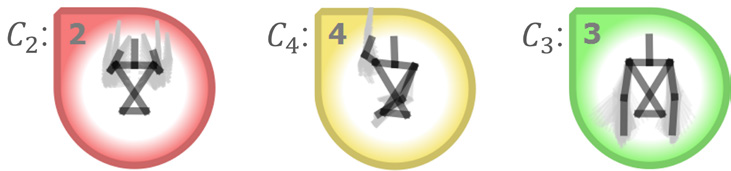
\includegraphics[width=.7\linewidth]{clus-MotionFlow}
	\caption[Visual representation of human pose clusters]{Visual representation of human pose clusters. The dark gray stick figure represents the centroid of the cluster, and other light gray ones indicate other poses in the cluster. \is{Jang2016}}
	\label{fig:lr-MotionFlow}
\end{figure}

MotionFlow then uses a force-directed graph of clusters to illustrate their relationship with node distance mapping to the similarity of pose clusters and edges indicating the directed transition between two clusters. Edges are color coded to represent the transition frequency. A user is allowed to interactively change the number of clusters, enabling exploration of the dataset. However, the re-clustering process may change all existing clusters and make it difficult for the user to keep track. To address this issue, MotionFlow allows the user to select the clusters to be locked or unchanged during the re-clustering process. He or she is also able to interactively merge or split clusters according to his or her own assessment.

Similarly, to provide an overall understanding of human motion tracking data, MotionExplorer~\cite{Bernard2013} applies a hierarchical clustering method~\cite{Han2011}, which seeks to build a hierarchy of clusters. MotionExplorer takes a divisive approach considering all data items starting within the same cluster and splitting them until a termination condition is met. One of the important decisions in this clustering technique is to determine which cluster to split next. The user is allowed to choose among several splitting strategies such as \emph{maximum standard deviation} to split the most varied cluster first and \emph{highest number of elements} to split the largest cluster first. The hierarchy is visualized as a dendrogram as in \autoref{fig:lr-MotionExplorer}. Clusters are obtained by cutting the dendrogram at the desired vertical level: each connected branch forms a cluster. The vertical axis of the dendrogram can encode different variables depending on the splitting strategy. In \autoref{fig:lr-MotionExplorer}, it shows the standard deviation of each cluster and the user is allowed to slide the cutting value to adjust the resulting clusters.

\begin{figure}
	\centering
	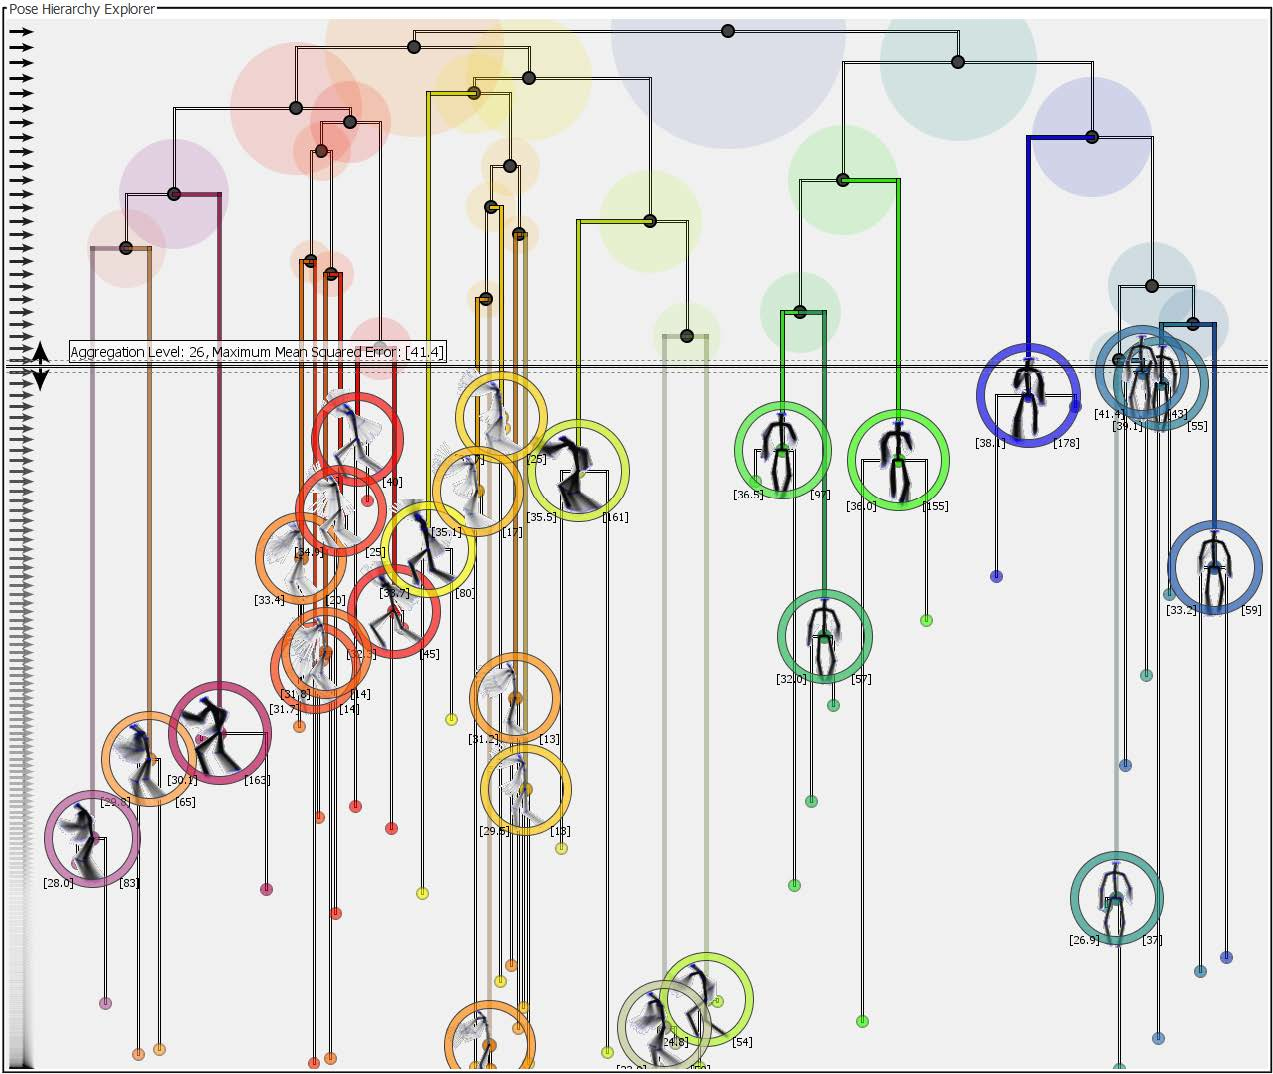
\includegraphics[width=.8\linewidth]{clus-MotionExplorer}
	\caption[A divisive hierarchical clustering of human poses]{A divisive hierarchical clustering of human poses visualized as a dendrogram. Clusters are connected branches after the dendrogram is cut at the desired vertical level. \is{Bernard2013}}
	\label{fig:lr-MotionExplorer}
\end{figure}

A different approach in hierarchical clustering is bottom-up or agglomerative clustering. The process starts with singleton clusters before merging the most similar clusters together until a termination condition is met. NewsLab~\cite{Ghoniem2007} applies such an approach in analysis of large scale broadcast news video collections. It builds a hierarchy of clusters over all keywords extracted from available video captions based on their co-occurrences in the news stories. Therefore, strongly correlated keywords are grouped into the same clusters whereas loosely related keywords are separated in different clusters. Each cluster is visualized as a stream showing the evolution of the keywords within the cluster over time with closely related clusters placed close to each other to allow navigation to different depths of the cluster hierarchy (\autoref{fig:lr-NewsLab}).

\begin{figure}
	\centering
	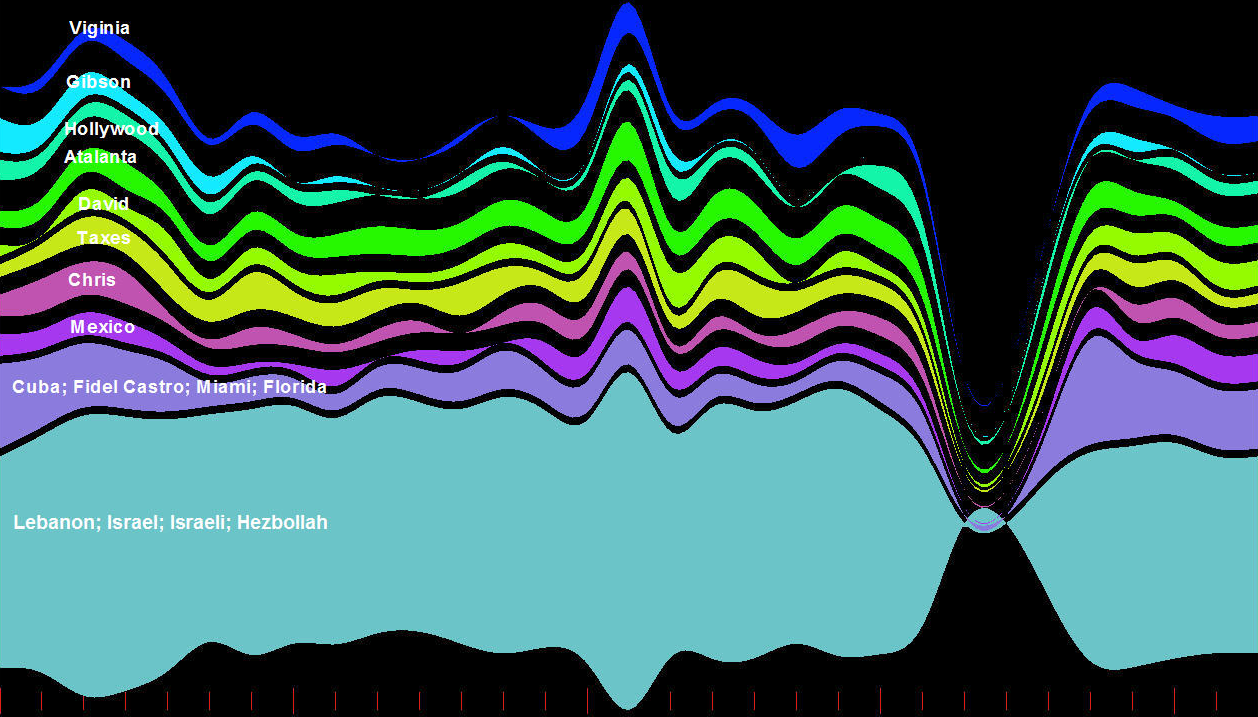
\includegraphics[width=.8\linewidth]{clus-NewsLab}
	\caption[An agglomerative hierarchical clustering of video captions]{An agglomerative hierarchical clustering of video captions visualized as streams. Each cluster is a colored stream, with related clustered placed close together. \is{Ghoniem2007}}
	\label{fig:lr-NewsLab}
\end{figure}

Understanding human movement patterns in both space and time plays an important role in urban planing. Analysis and presentation of large and complex datasets that contain a number of people in different places and their movement between those places over time are challenging. Mobility Graphs~\cite{Landesberger2016} applies cluster analysis to simplify the data in both spatial and temporal dimensions to gain an overall understanding of the datasets. First, it aggregates places using a density-based clustering technique that considers both the density of places and their flow magnitudes so that close and highly connected can be grouped together. Then, a temporal aggregation algorithm groups the time steps by the similarity of those simplified places using a k-means clustering technique. \autoref{fig:lr-MobilityGraphs} shows 7 temporal clusters of simplified places. The clusters are color coded with a calendar view to reveal temporal patterns over a week. In each cluster, a node shows an aggregated place with size corresponding to the total number of people in all individual places and arrow widths representing the number of people moving between two aggregated places.

\begin{figure}
	\centering
	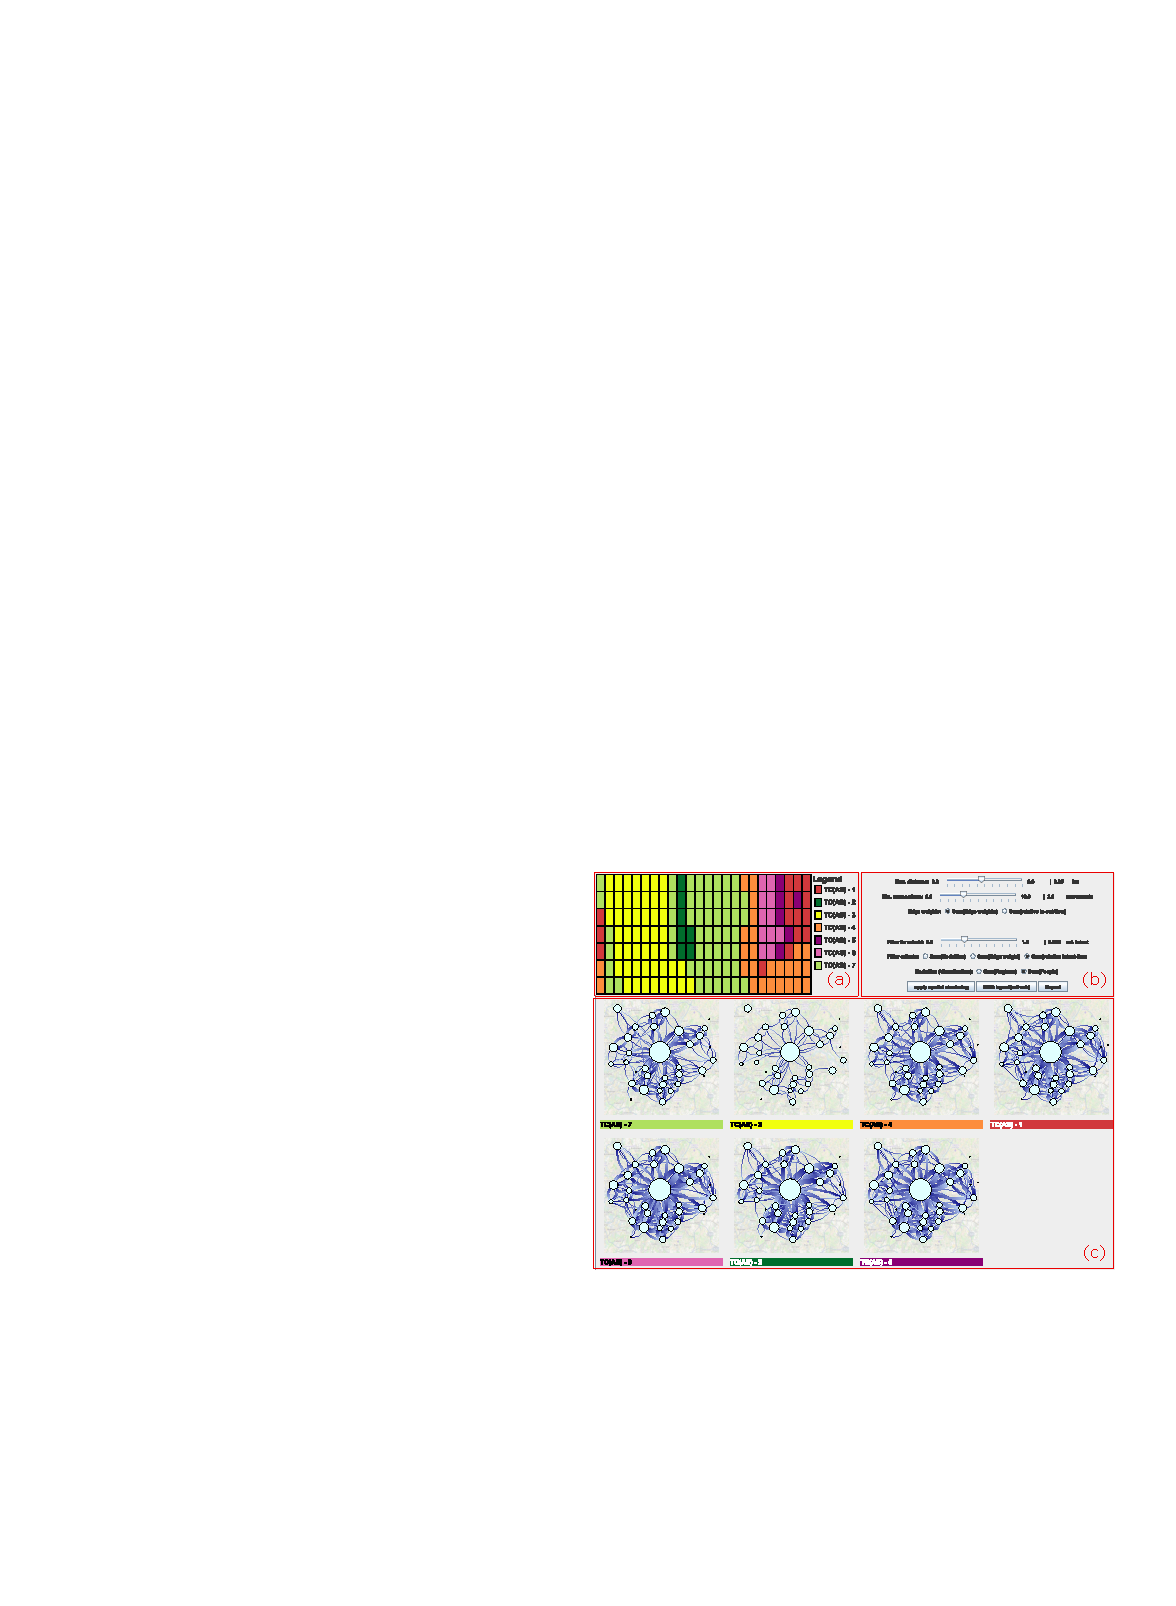
\includegraphics[width=.8\linewidth]{clus-MobilityGraphs}
	\caption[Spatial and temporal aggregation of movement data]{Spatial and temporal aggregation of movement data. Seven temporal clusters of simplified places are shown and color coded together with a calendar view to reveal daily pattern. \is{Landesberger2016}}
	\label{fig:lr-MobilityGraphs}
\end{figure}

\subsubsection{Classification}
\paragraph{Overview}
Classification predicts the value of a categorical (discrete or nominal) attribute based on the values of other attributes. It builds a model (or \emph{classifier}) based on a labeled training dataset (i.e., \emph{supervised learning}) and applies it in labeling new data~\cite{Han2011}. The model needs to not only identify the labels in the training dataset well but also be general enough to predict the labels of new data correctly. One common and intuitive classification algorithm is decision tree induction~\cite{Quinlan1986}. Each non-leaf node of the tree represents a ``test'' on an attribute, which splits the node to multiple branches, each for an outcome of the test. Each leaf node is associated with a class label and is the result of a sequence of tests starting from the root node.

The importance of building a decision tree is choosing which attribute to split at each node. Intuitively, we should choose attributes that can divide nodes into ``pure'' child nodes so that all data items in a child node belong to a single class and no further splits are needed. For example, in a binary classification, consider a training dataset with 10 records, 5 labeled ``true'' and 5 labeled ``false''. Attribute $A1$ splits the set to two subsets: (5 ``true'', 0 ``false'') and (0 ``true'', 5 ``false''). Attribute $A2$ splits the set to (3 ``true'', 2 ``false'') and (2 ``true'', 3 ``false''). The subsets split by $A1$ is ``purer'' than the one by $A2$ because they do not contain a mix of ``true'' and ``false''. To achieve this purity, several attribute measurements have been proposed such as \emph{information gain} and \emph{gini index}~\cite{Tan2006}. More detailed analysis of these measurements and other classification algorithms are out of the scope of this thesis and can be found in data mining textbooks~\cite{Tan2006,Han2011}.

\paragraph{Application Examples}
Exploring a large image collection is challenging. Besides the low-level visual features, the semantic contents of images are also effective in searching for relevant ones. Image classification techniques can be used to extract such semantic contents. For example, Fan~et~al.~\cite{Fan2004} detect salient objects in images and associate them with predefined semantic contents according to their perceptual properties. Similar contents are then grouped into a higher level semantic concept; for instance, ``sand field'', ``sea water'' and ``boat'' salient objects construct the concept of ``sea world''. Visualization can make the output of classification algorithms more interpretable and interactive. To provide an overview of an image collection, Yang~et~al.~\cite{Yang2006} shows the extracted semantic contents, with each as a glyph, in a 2D display so that related contents are located close together using a multidimensional dimension scaling method~\cite{Borg2005}. Similarly, images are also displayed based on their similarity as in \autoref{fig:lr-SIBa}. Zooming and panning are provided to make the visualization more scalable. When an image is selected, the visualization can be switched to a \emph{rainfall} mode, in which the selected image is shown at the bottom and related images are stacked above it based on their similarity with the selected one (\autoref{fig:lr-SIBb}). Users are allowed to reassign the contents computed for each image; however, the model does not take into account the changes to improve its accuracy when classifying new images.

\begin{figure}
\centering
\subcaptionbox{Multidimensional dimension scaling view of images.\label{fig:lr-SIBa}}[.47\columnwidth]{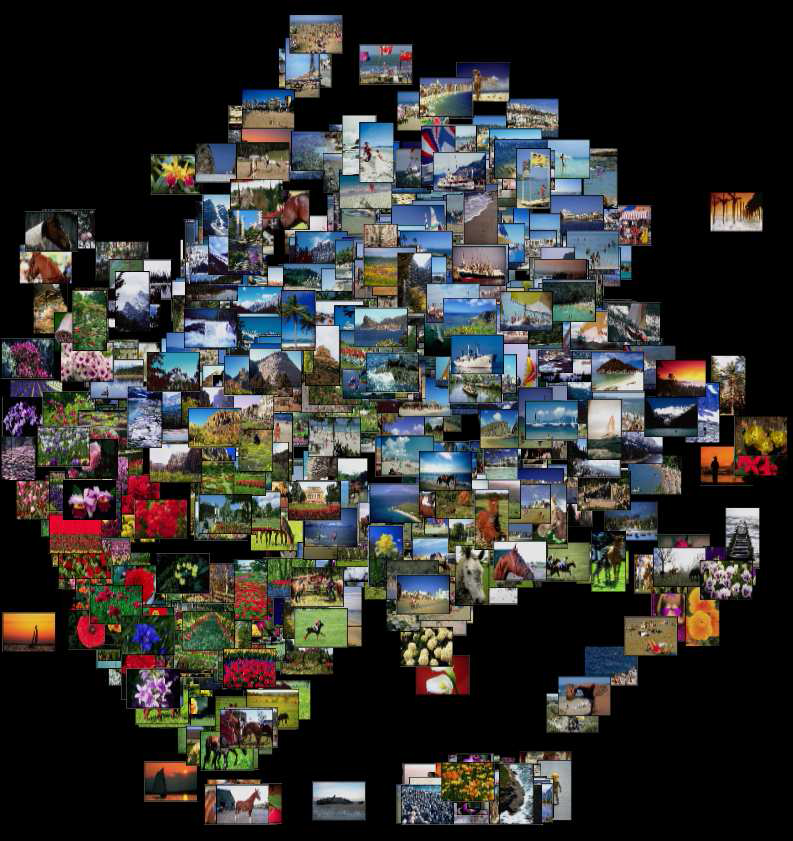
\includegraphics[height=.47\columnwidth]{clas-SIBa}}
\hfill
\subcaptionbox{Rainfall view of a selected image with highly related images at the bottom.\label{fig:lr-SIBb}}[.47\columnwidth]{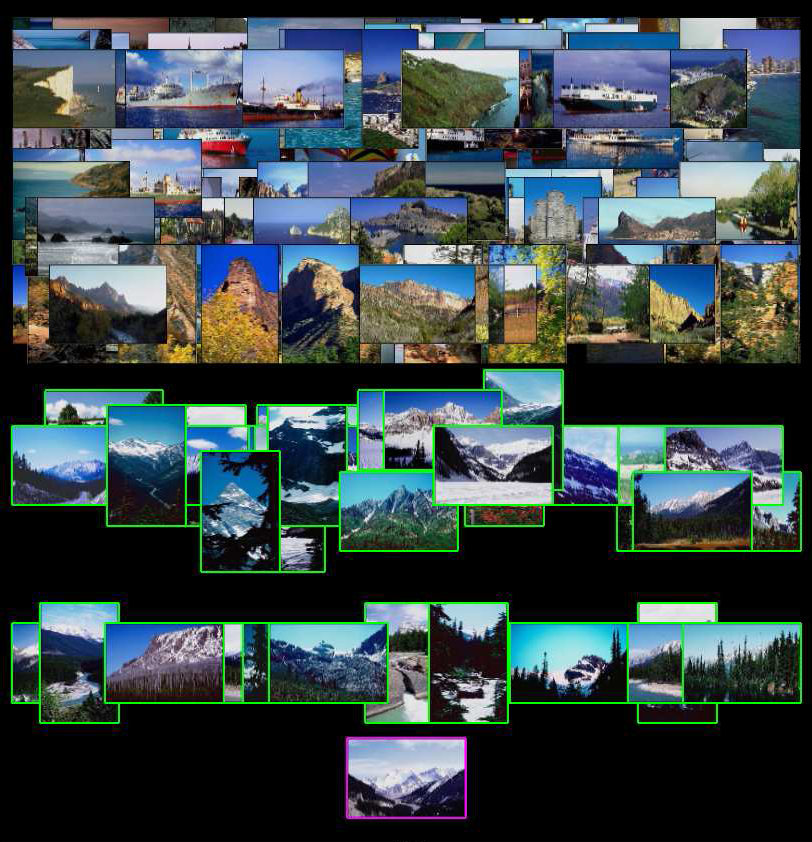
\includegraphics[height=.47\columnwidth]{clas-SIBb}}
\label{fig:lr-SIB}
\caption[Large-scale image browser using classification]{Large-scale image browser with semantic content-based image classification. \is{Yang2006}}
\end{figure}

In a binary classification, the classifier output is either \emph{positive} or \emph{negative}. Two types of error can happen including \emph{false positive} (classified as positive but the actual class is negative) and \emph{false negative} (classified as negative but the actual class is positive). Depending on a particular domain, the costs of these error types might be considerably different. For example, wrong prediction of a healthy patient with a cancer has a much lower impact than missing a patient with a real cancer. Migut and Worring~\cite{Migut2010} allow users to adjust the trade-off between these two error types through a visualization of the classification model as shown in \autoref{fig:lr-Migut}.

\begin{figure}
\centering
\subcaptionbox{Performance curve of the classification model with horizontal axis showing the false positive rate and vertical axis showing the false negative rate.\label{fig:lr-Migut1}}[\columnwidth]{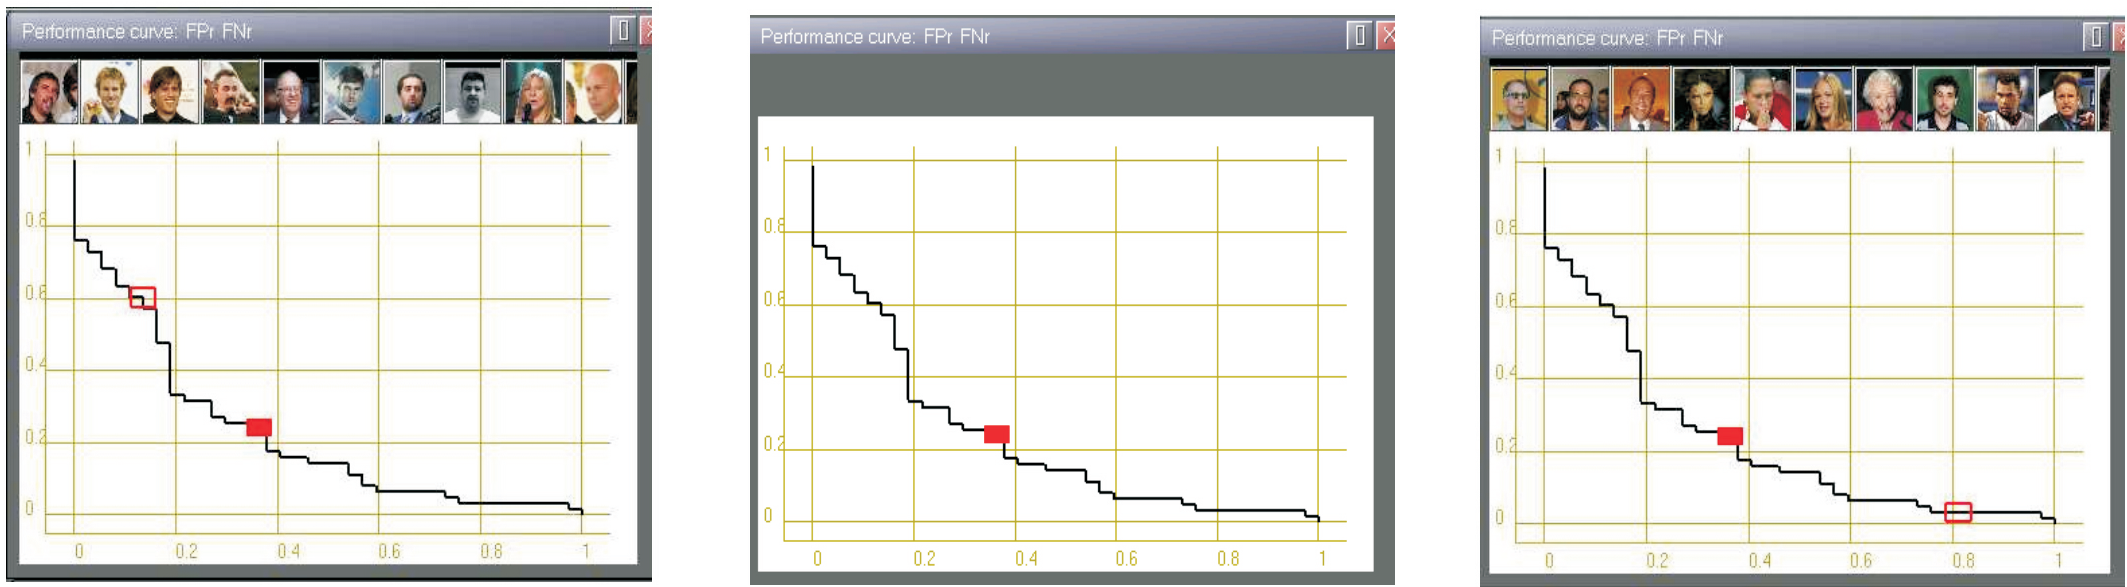
\includegraphics[width=\columnwidth]{clas-Migut1}}
\\
\subcaptionbox{Data with color indicating original class and size showing classification accuracy.\label{fig:lr-Migut2}}[\columnwidth]{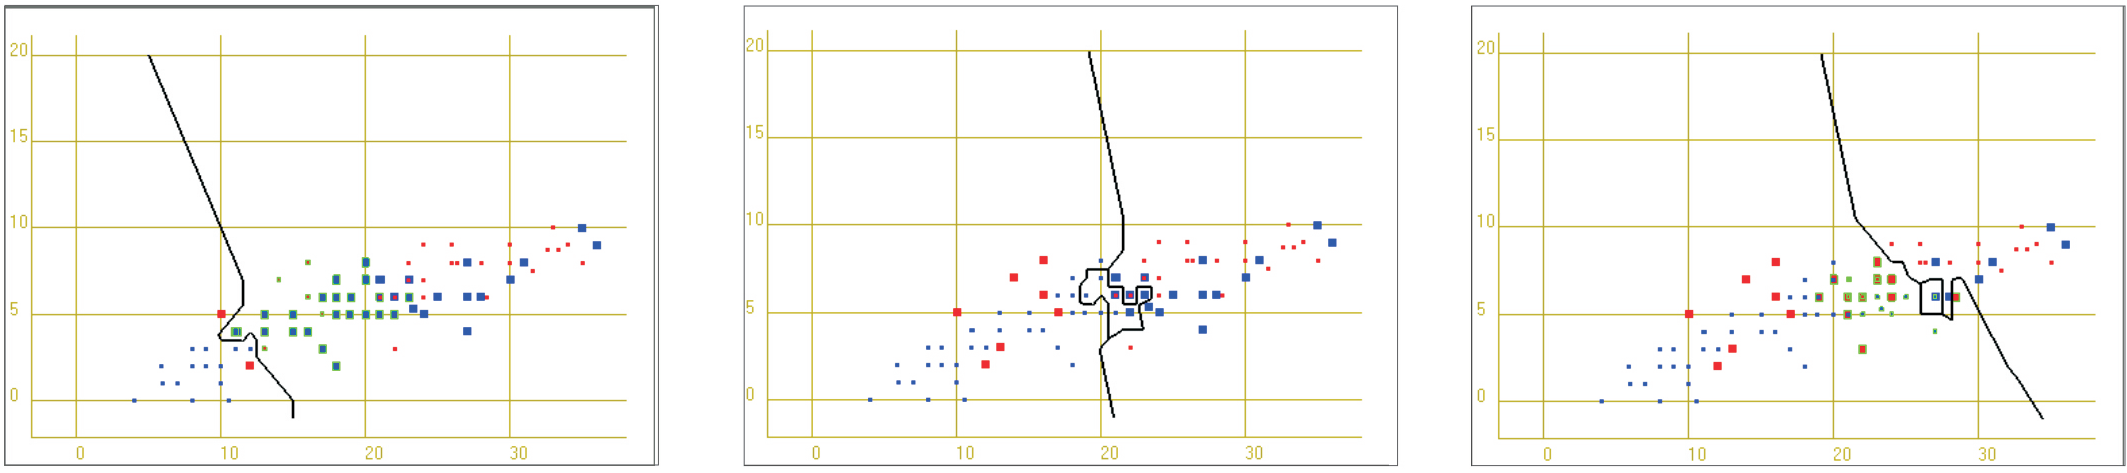
\includegraphics[width=\columnwidth]{clas-Migut2}}
\caption[Visualization and interaction of a classification model]{Visualization and interaction of a classification model. Middle figures show the initial state of the system, with initial operating point on the performance curve and corresponding data scatter plot. Left figures show the state of the system when an expert manipulates the operating point to include more false negatives and on the right to include more false positives. \is{Migut2010}}
\label{fig:lr-Migut}
\end{figure}

Typically, a receiver operating characteristic curve~\cite{Fawcett2006} is used to illustrate the performance of a binary classifier when its discrimination threshold is varied. The curve is composed from a set of true positive rate and false positive rate pairs at various threshold values. Migut and Worring replace the true positive rate with the false negative rate (\autoref{fig:lr-Migut1}) because their focus is comparing trade-off between the two error rates. Numerical data is visualized in a scatter plot with the decision boundary separating a 2D plane into two regions, each for a class (\autoref{fig:lr-Migut2}). For each data point, color shows the original class and size indicates the accuracy of the classified class. The current classification setting is shown as a red point on the performance curve, and the user is allowed to move that point along the curve to change the false positive and false negative rates. The classification reruns with the new threshold and rates and updates on the data scatter plot.

Classification requires training data; however, it can be time-consuming and laborious to produce such a dataset. ScatterBlogs2~\cite{Bosch2013} includes an interactive classifier that speeds up the training data labeling and classifier construction before applying it in real-time monitoring messages of interest. First, the user can search for relevant messages using a standard keyword query. The system then highlights non-trivial terms that frequently co-occur with the original keywords. The result set of highly relevant messages can be used as \emph{positive} samples, whereas some arbitrary messages not returned in the result set can be used as \emph{negative} ones. After creating an initial classifier, the user can inspect messages to correct and update the classifier through the message visualization. Messages are shown in a map as a colored glyph with color hue indicating class and brightness showing classification confidence (\autoref{fig:lr-ScatterBlogs2}). They can be filtered by confidence, allowing the user to focus on ones with less certainty, which need a human expert to verify.

\begin{figure}
	\centering
	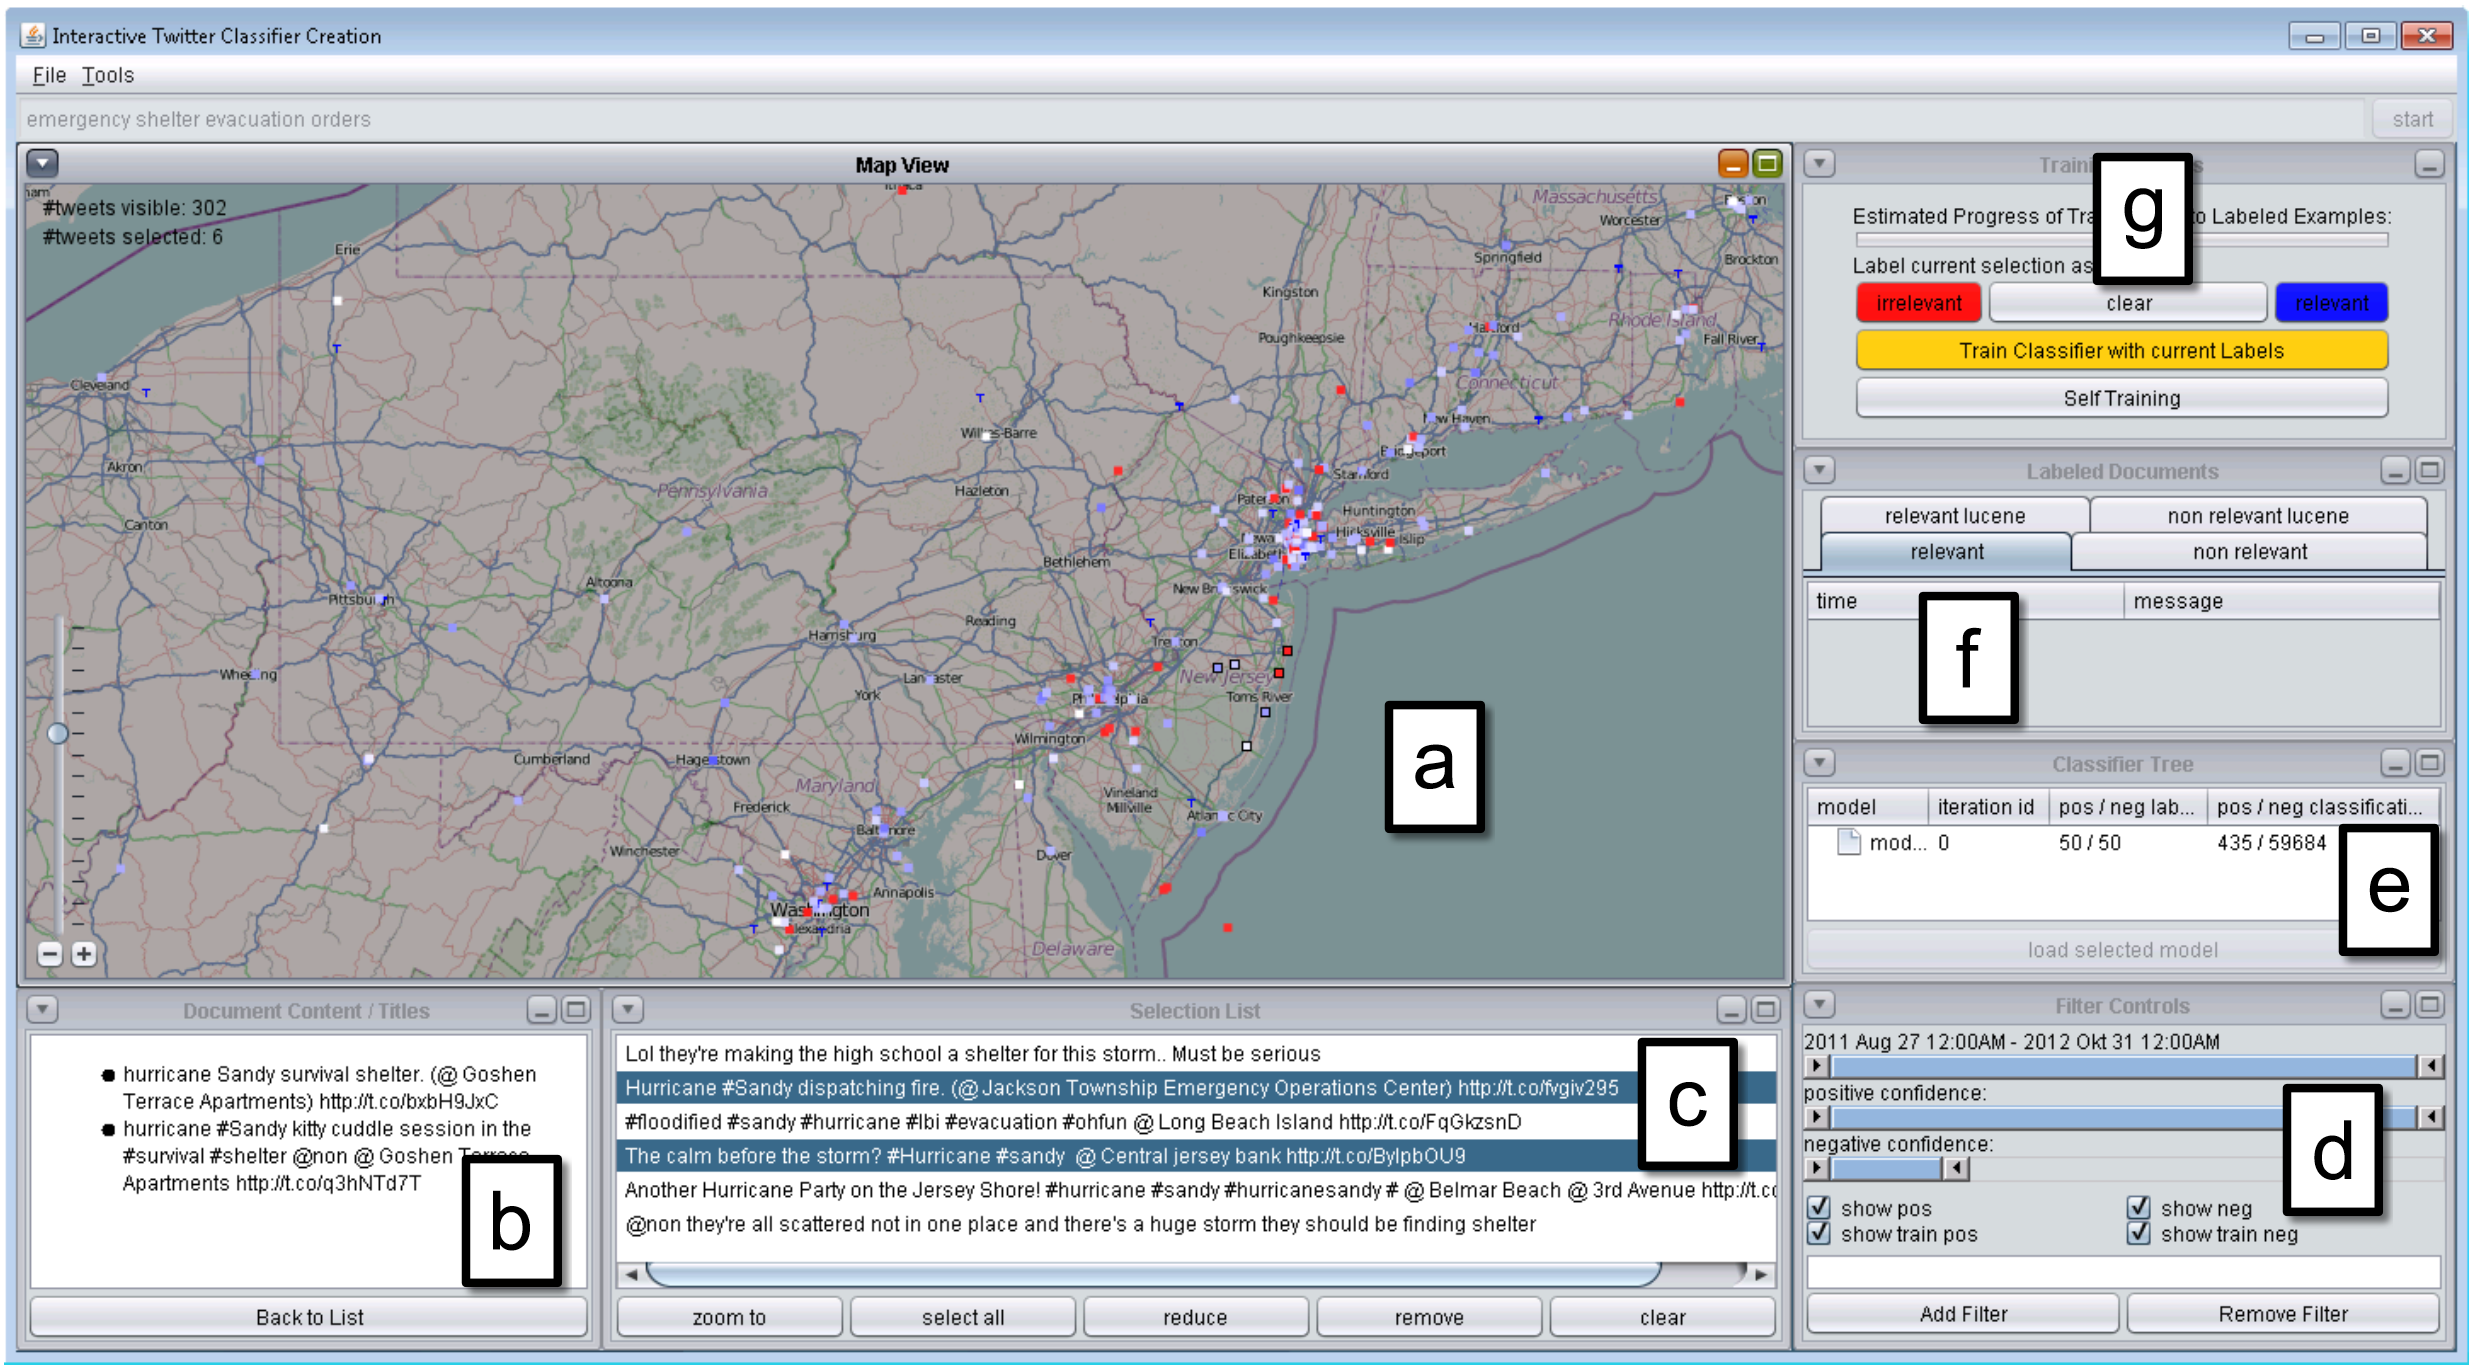
\includegraphics[width=\linewidth]{clas-ScatterBlogs2}
	\caption[ScatterBlogs2 -- interactive classifier]{ScatterBlogs2 speeding up the creation of a classifier through interactive visualization. \is{Bosch2013}}
	\label{fig:lr-ScatterBlogs2}
\end{figure}

An essential step in classification of high dimensional datasets is feature selection, which selects a subset of relevant features for use in model construction without much loss of information. This step also simplifies the model and reduces training time. INFUSE~\cite{Krause2014} supports users to explore the predictive power of features in their models. The system allows comparison of features across four feature selection algorithms. Each feature is shown as a circle glyph divided into four equal quadrants, each for an algorithm (\autoref{fig:lr-INFUSE}). A quadrant is further split into 10 slices, each for a cross-validation fold (or random subset of data) to ensure the result  robust. The length of a slice indicates the rank of that feature using a given algorithm. Therefore, a glyph can show how its feature performs in different algorithms. To provide an overview of all features, INFUSE shows multiple glyphs in either a sequential layout or a scatter plot, where different options can be used for axes such as average rank of a feature or a more sophisticated importance measurement. It also allows users to explore four classification algorithms by showing the score of all 16 combination of feature selection and classification algorithms. More importantly, users are allowed to build their own model by selecting features besides the ones produced by the four given algorithms. The custom feature set is then included in the classification score comparison.

\begin{figure}
	\centering
	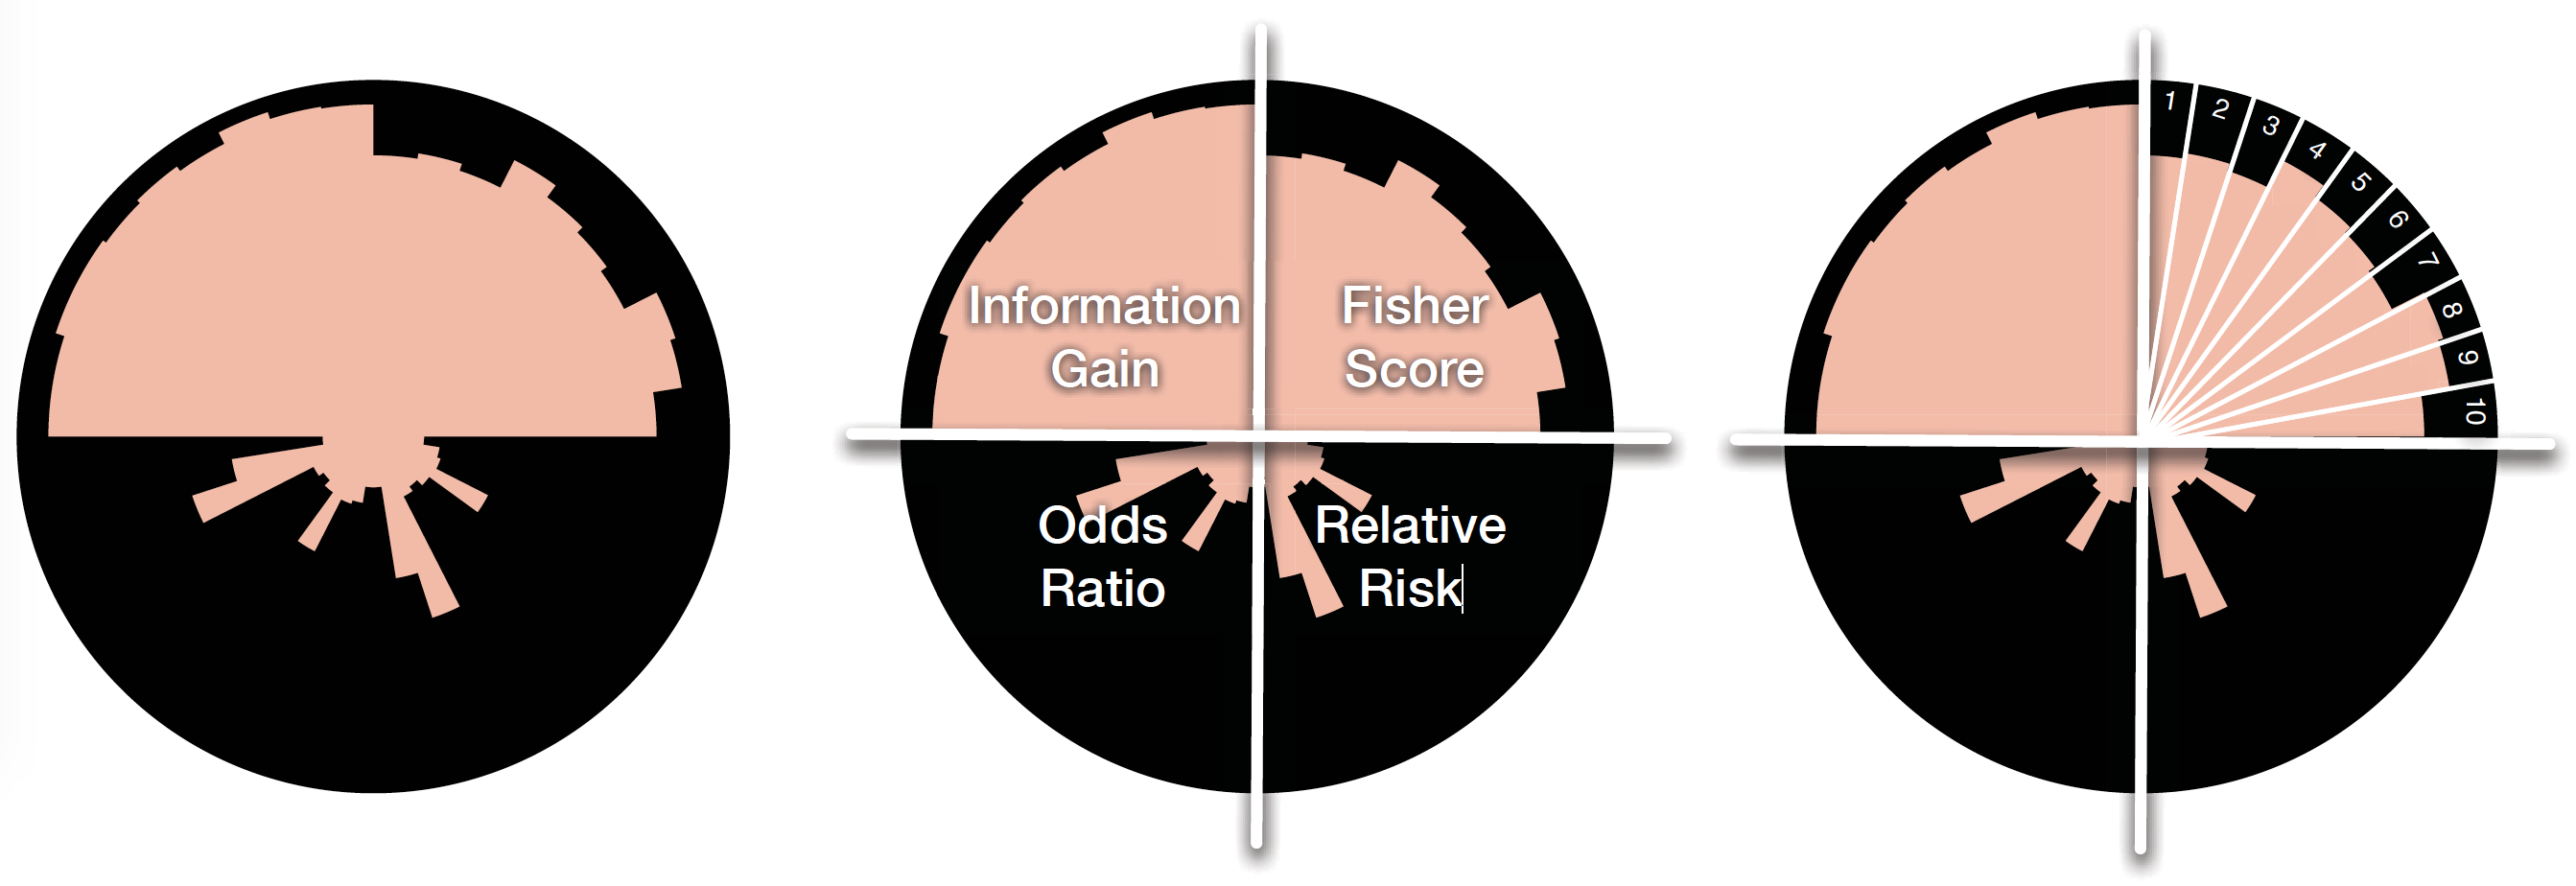
\includegraphics[width=.8\linewidth]{clas-INFUSE}
	\caption[INFUSE -- comparison of features in classification]{INFUSE allowing comparison of feature selection and classification algorithms. The circle glyph is divided into 4 quadrants, each for a feature selection algorithm. Each quadrant is further split into 10 slices, each for a cross-validation fold. \is{Krause2014}}
	\label{fig:lr-INFUSE}
\end{figure}

\subsection{Evaluation Methods}
\label{sub:lr-evaluation}
A visualization, no matter how novel and interesting it is, needs to be evaluated to check whether it meets the design goals and supports the target users to complete the intended tasks. Evaluation has been a research topic in visualization as the field becomes more mature~\cite{Plaisant2004}. Excellent reviews of visualization evaluation are available with different perspectives such as evaluation techniques~\cite{Carpendale2008}, scenarios~\cite{Lam2012} and design process~\cite{Munroe2009}.

In this section, we review the evaluation techniques based on the visualization design model by Munzner~\cite{Munroe2009}, helping address different concerns separately. The model consists of four levels including explaining the tasks and available data in the vocabulary of the problem domain, abstracting them into domain-independent operations and data types, designing visual encoding and interaction techniques to solve the abstract tasks, and developing algorithms to execute these techniques efficiently. Each level has its own \emph{threats} to validity and methods to address them. Two types of methods are distinguished: \emph{immediate} approaches can be done before inner levels are implemented, whereas \emph{downstream} approaches requires all inner levels are completed. The threats and evaluation methods for all levels are summarized in \autoref{fig:lr-nested-model}.

\begin{figure}
	\centering
	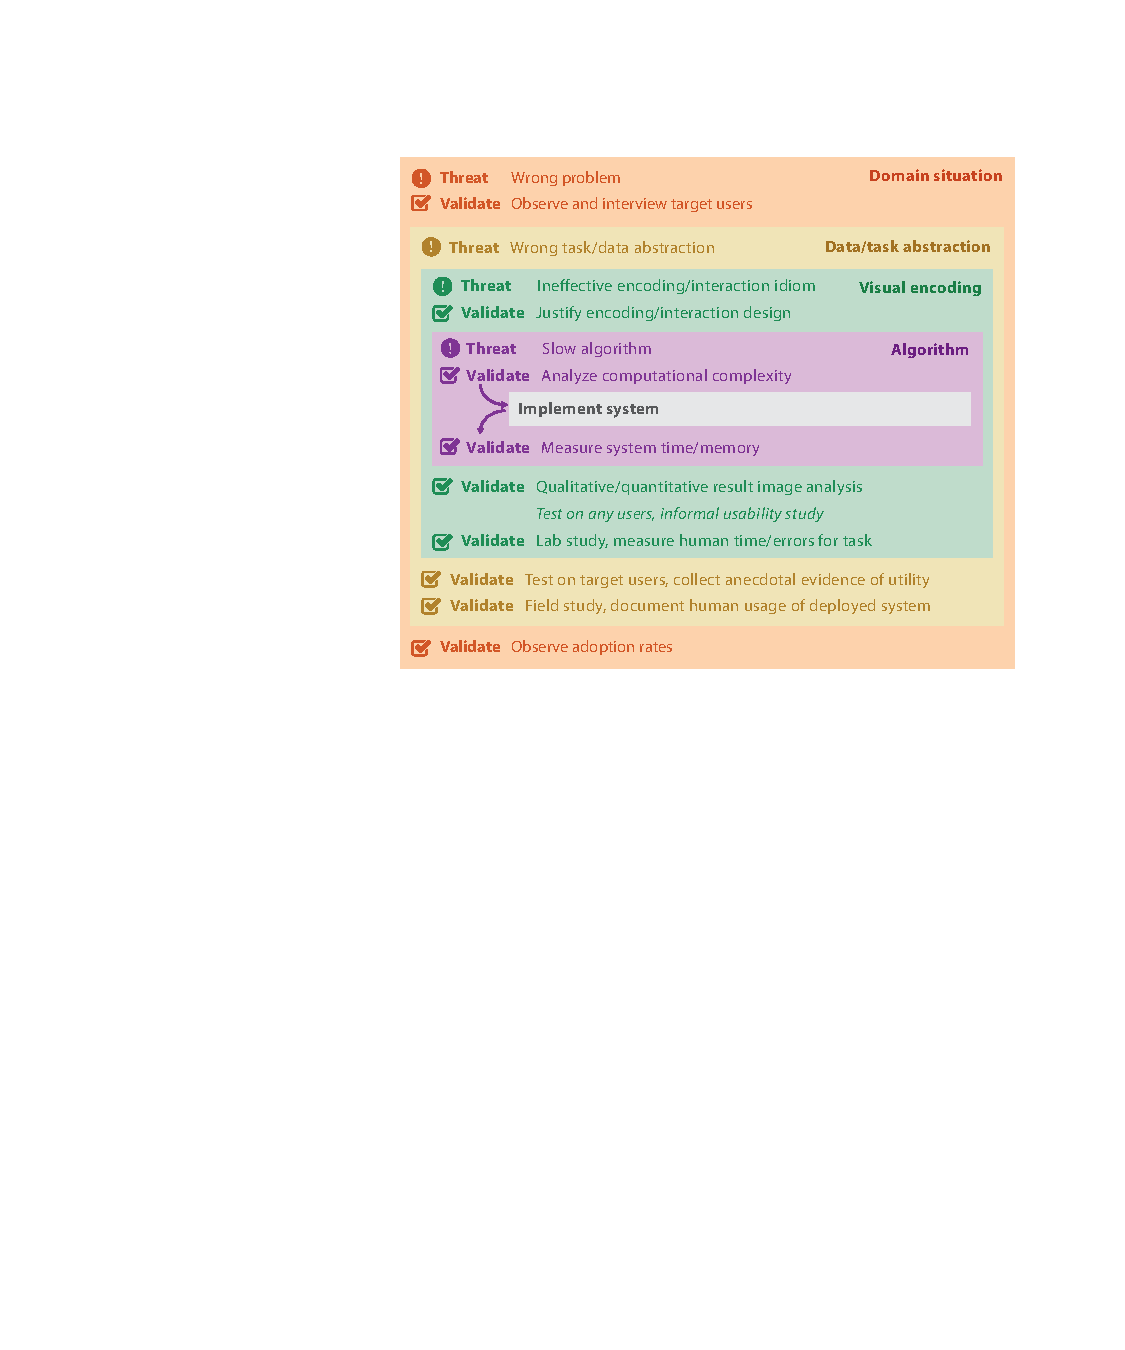
\includegraphics[width=.8\linewidth]{nested-model}
	\caption[Nested validation model of visualization design]{Threats and validation at each of the four nested levels of visualization design. \is{Munzner2014}}
	\label{fig:lr-nested-model}
\end{figure}

\subsubsection{Domain Problem and Data Characterization}
The domain problem of target users is investigated to see if visualization is a potential solution. The primary threat is that the problem is mischaracterized: the users do not really suffer from the identified problem. An immediate form of validation is \emph{field study}~\cite{Carpendale2008}, where the investigator observes how target users act in real-world settings in order to learn and verify the characterization. Another technique is \emph{contextual inquiry}~\cite{Holtzblatt1993}, which allows the investigator to occasionally interview while the user is engaged in the process. One example is the study by Sedlmair~et~al.~\cite{Sedlmair2008} on current working behavior and environments of automotive analysis and diagnosis experts.

One downstream form of validation is to report the adoption rate of the tool by the target users. High effort is required to make the visualization solution reliable and deployable in the real-world environment. Examples include a field study of Google's Notebook product~\cite{Russell2008} and 6-week field trial of SparTag.us -- a tagging system for foraging web content~\cite{Hong2008}.

\subsubsection{Operation and Data Type Abstraction}
The threat at this level is the identified data and task abstraction do not solve the characterized problem. Only downstream approaches can be used to validate the abstraction. The deployed system needs to be used by target users completing their routine tasks in real-world environment. The goal of this evaluation is to collect anecdotal evidence that the solution is in fact useful. The observation and interview need to focus on understanding how the tool is used, and how it helps or hinders the users in performing their tasks. An example is a longitudinal field study of LiveRAC system that supports analysis of system management time-series data~\cite{McLachlan2008}.

Evaluating visualization for supporting sensemaking can be done at this level, as the \emph{evaluating visual data analysis and reasoning} scenario in the taxonomy by Lam~et~al.~\cite{Lam2012}. Due to the nature of sensemaking, evaluation is often carried out as case studies~\cite{Kang2011} with observation and interview, and followed by qualitative data analysis~\cite{Lazar2010}. Attempts also have been made to quantify the insight or knowledge gained during sensemaking~\cite{Wilson2013}.

\subsubsection{Visual Encoding and Interaction Design}
At this level, the threat is that the chosen design becomes ineffective at communicating the desired abstraction to the user. One immediate form of validation is to justify every design decision based on known design principles such as the ones discussed in \autoref{sub:lr-design}, or more comprehensive predefined guidelines as in heuristic evaluation~\cite{Zuk2006}. Asking experts to review the design prototype also provides valuable feedback~\cite{Tory2005}.

A common downstream approach is to conduct a controlled experiment comparing the design with other state-of-the-art alternatives~\cite{Xu2012}. A number of participants, depending on the  expected size of the experiment, carry out a number of tasks representing real-world cases. Typically, task completion time and accuracy are measured and analyzed using hypothesis testing methods~\cite{Field2003}. Post-task interviews are often combined to establish deeper understanding about how the visualization is used. If the experiment can be completed online, a crowd-sourcing approach using Amazon's Mechanical Turk service can help largely increase the size of participants~\cite{Heer2010a}. Another downstream approach is the measurement of common aesthetic metrics such as the number of edge crossings and edge bends that have been used in graph visualization~\cite{Sugiyama1981}.

\subsubsection{Algorithm Design}
The primary threat at this level is the algorithm is suboptimal in terms of time or memory performance. In interactive visualization, it is essential to ensure the interaction responsive in real-time. Analyzing the complexity of the algorithm using the standard approaches from the computer science literature~\cite{Cormen2009} is an intermediate form of validation. The complexity can be computed based on the size of dataset or the display screen. Downstream approaches include measuring running time and memory usage for benchmark datasets.

%http://www.cc.gatech.edu/~stasko/papers/vast09-eval.pdf
%https://www.purdue.edu/discoverypark/vaccine/assets/pdfs/publications/pdf/Beyond%20Usability.pdf
%http://www.cc.gatech.edu/~stasko/7450/Papers/fekete08.pdf
%https://www.cs.ubc.ca/~tmm/courses/cpsc533c-05-fall/readings/vov.pdf

\subsection{Summary}
Visualization helps people carry out tasks more effectively by amplifying human cognition through visual representation and interaction. Visual analytics includes automated analysis techniques to help make sense of complex datasets. This thesis contributes novel visualization techniques and systems to support the sensemaking process. The visualizations are designed based on a number of principles and guidelines described in this chapter such as Gestalt laws, color mapping and fluid interaction. The designs are implemented and evaluated rigorously with suitable methods as discussed previously. The visualizations make use of the provenance data captured during the sensemaking process. Next, we will discuss the literature on capture and visualization of provenance data.